%%%%%%%%%%%%%%%%%%%%%%%%%%%%%%%%%%%%%%%%%%%%%%%%%%%%%%%%%%%%%%%%%
%                                                               % 
%%%%%%%%%%%%%%%%%%%%%%%%%%%%%%%%%%%%%%%%%%%%%%%%%%%%%%%%%%%%%%%%%
\documentclass{dmathesis}
%% uncommand the following line to print equation labels next to
%% equation numbers. 
%% (left commented: it prints every \label name inside the text)
%\usepackage{showlabel}
%% The following is to control the format of your thesis
%%%%%%%%%%%%%%%%%%%%%%%%%%%%%%%%%%%%%%%%%%%%%%%%%%%%%%%%%%%%%%%%%%%%%%%%%%
%     This is format.tex file needed for the dmathesis.cls file.  You    %
%  have to  put this file in the same directory with your thesis files.  %
%                Written by M. Imran 2001/06/18                          % 
%                 No Copyright for this file                             % 
%                 Save your time and enjoy it                            % 
%                                                                        % 
%%%%%%%%%%%%%%%%%%%%%%%%%%%%%%%%%%%%%%%%%%%%%%%%%%%%%%%%%%%%%%%%%%%%%%%%%%
%%%%%  Put packages you want to use here and 'fancyhdr' is required   %%%%
%%%%%%%%%%%%%%%%%%%%%%%%%%%%%%%%%%%%%%%%%%%%%%%%%%%%%%%%%%%%%%%%%%%%%%%%%%
\usepackage{fancyhdr}
\usepackage{epsfig}
\usepackage{cite}
\usepackage{graphicx}
\usepackage{amsmath}
\usepackage{theorem}
\usepackage{amssymb}
\usepackage{latexsym}
\usepackage{epic}
\usepackage{nomencl}
\usepackage{nomencl}
\usepackage{titlesec}
% Chapter spacing (fix gap from header)
\titlespacing*{\chapter}{0pt}{-60pt}{10pt}

% Section spacing (gap before & after section title)
\titlespacing*{\section}{0pt}{10pt}{5pt}
\titlespacing*{\subsection}{0pt}{5pt}{3pt}


\makenomenclature
 
\renewcommand{\nomname}{List of Abbreviations}
%%%%%%%%%%%%%%%%%%%%%%%%%%%%%%%%%%%%%%%%%%%%%%%%%%%%%%%%%%%%%%%%%%%%%%%%%%
%%%%%                 Set line spacing = 1.5 here                   %%%%%%
%%%%%%%%%%%%%%%%%%%%%%%%%%%%%%%%%%%%%%%%%%%%%%%%%%%%%%%%%%%%%%%%%%%%%%%%%%
\renewcommand{\baselinestretch}{1.5}
%%%%%%%%%%%%%%%%%%%%%%%%%%%%%%%%%%%%%%%%%%%%%%%%%%%%%%%%%%%%%%%%%%%%%%%%%%
%%%%%                      Your fancy heading                       %%%%%%
%%%%% For the final copy you need to remove '\bfseries\today' below %%%%%%
%%%%%%%%%%%%%%%%%%%%%%%%%%%%%%%%%%%%%%%%%%%%%%%%%%%%%%%%%%%%%%%%%%%%%%%%%%
\pagestyle{fancy}
\renewcommand{\chaptermark}[1]{\markright{\chaptername\ \thechapter.\ #1}}
\renewcommand{\sectionmark}[1]{\markright{\thesection.\ #1}{}}
\lhead[\fancyplain{}{}]%
      {\fancyplain{}{\bfseries\rightmark}}
\chead[\fancyplain{}{}]%
      {\fancyplain{}{}}
\rhead[\fancyplain{}{}]%
      {\fancyplain{}{\bfseries\thepage}}
\lfoot[\fancyplain{}{}]%
      {\fancyplain{}{}}
\cfoot[\fancyplain{}{}]%
      {\fancyplain{}{}}
\rfoot[\fancyplain{}{}]%
{\fancyplain{}{\bfseries}}
%%%%%%%%%%%%%%%%%%%%%%%%%%%%%%%%%%%%%%%%%%%%%%%%%%%%%%%%%%%%%%%%%%%%%%%%%%
%%%%%%%%%%%%Here you set the space between the main text%%%%%%%%%%%%%%%%%%
%%%%%%%%%%%%%%%%%%%and the start of the footnote%%%%%%%%%%%%%%%%%%%%%%%%%%
%%%%%%%%%%%%%%%%%%%%%%%%%%%%%%%%%%%%%%%%%%%%%%%%%%%%%%%%%%%%%%%%%%%%%%%%%%
\addtolength{\skip\footins}{5mm}
%%%%%%%%%%%%%%%%%%%%%%%%%%%%%%%%%%%%%%%%%%%%%%%%%%%%%%%%%%%%%%%%%%%%%%%%%%
%%%%%      Define new counter so you can have the equation           %%%%%
%%%%%    number 4.2.1a for example, this a gift from J.F.Blowey      %%%%%
%%%%%%%%%%%%%%%%%%%%%%%%%%%%%%%%%%%%%%%%%%%%%%%%%%%%%%%%%%%%%%%%%%%%%%%%%%
\newcounter{ind}
\def\eqlabon{
\setcounter{ind}{\value{equation}}\addtocounter{ind}{1}
\setcounter{equation}{0}
\renewcommand{\theequation}{\arabic{chapter}%
         .\arabic{section}.\arabic{ind}\alph{equation}}}
\def\eqlaboff{
\renewcommand{\theequation}{\arabic{chapter}%
         .\arabic{section}.\arabic{equation}}
\setcounter{equation}{\value{ind}}}
%%%%%%%%%%%%%%%%%%%%%%%%%%%%%%%%%%%%%%%%%%%%%%%%%%%%%%%%%%%%%%%%%%%%%%%%%%
%%%%%%%%%%%%           New theorem you want to use              %%%%%%%%%%
%%%%%%%%%%%%%%%%%%%%%%%%%%%%%%%%%%%%%%%%%%%%%%%%%%%%%%%%%%%%%%%%%%%%%%%%%%
{\theorembodyfont{\rmfamily}\newtheorem{Pro}{{\textbf Proposition}}[section]}
{\theorembodyfont{\rmfamily}\newtheorem{The}{{\textbf Theorem}}[section]}
{\theorembodyfont{\rmfamily}\newtheorem{Def}[The]{{\textbf Definition}}}
{\theorembodyfont{\rmfamily}\newtheorem{Cor}[The]{{\textbf Corollary}}}
{\theorembodyfont{\rmfamily}\newtheorem{Lem}[The]{{\textbf Lemma}}}
{\theorembodyfont{\rmfamily}\newtheorem{Exp}{{\textbf Example}}[section]}
\def\remark{\textbf{Remark}:}
\def\remarks{\textbf{Remarks}:}
\def\bproof{\textbf{Proof}: }
\def\eproof{\hfill$\Box$}
%%%%%%%%%%%%%%%%%%%%%%%%%%%%%%%%%%%%%%%%%%%%%%%%%%%%%%%%%%%%%%%%%%%%%%%%%%
%%%%%%%    Bold font in math mode, a gift from J.F.Blowey       %%%%%%%%%%
%%%%%%%%%%%%%%%%%%%%%%%%%%%%%%%%%%%%%%%%%%%%%%%%%%%%%%%%%%%%%%%%%%%%%%%%%%
\def\bv#1{\mbox{\boldmath$#1$}}
%%%%%%%%%%%%%%%%%%%%%%%%%%%%%%%%%%%%%%%%%%%%%%%%%%%%%%%%%%%%%%%%%%%%%%%%%%
%%%%%%%        New symbol which is not defined in Latex         %%%%%%%%%%
%%%%%%%                 a gift from J.F.Blowey                  %%%%%%%%%%
%%%%%%%%%%%%%%%%%%%%%%%%%%%%%%%%%%%%%%%%%%%%%%%%%%%%%%%%%%%%%%%%%%%%%%%%%%
% The Mean INTegral
% to be used in displaystyle
\def\mint{\textstyle\mints\displaystyle}
% to be used in textstyle
\def\mints{\int\!\!\!\!\!\!{\rm-}\ }
%
% The Mean SUM
% to be used in displaystyle
\def\msum{\textstyle\msums\displaystyle}
% to be used in textstyle
\def\msums{\sum\!\!\!\!\!\!\!{\rm-}\ }
%%%%%%%%%%%%%%%%%%%%%%%%%%%%%%%%%%%%%%%%%%%%%%%%%%%%%%%%%%%%%%%%%%%%%%%%%%
%%%%%%%%%%            Define your short cut here              %%%%%%%%%%%%
%%%%%%%%%%%%%%%%%%%%%%%%%%%%%%%%%%%%%%%%%%%%%%%%%%%%%%%%%%%%%%%%%%%%%%%%%%
\def\poincare{Poincar\'e }
\def\holder{H\"older }

\makeatletter
% Chapter title spacing
% Section spacing
\renewcommand{\section}{\@startsection{section}{1}{0pt}%
  {-5pt}  % space before
  {5pt}   % space after
  {\normalfont\Large\bfseries}}

% Subsection spacing
\renewcommand{\subsection}{\@startsection{subsection}{2}{0pt}%
  {-3pt}  % space before
  {3pt}   % space after
  {\normalfont\large\bfseries}}
\makeatother

\makeatletter

\def\@makechapterhead#1{%
  \vspace*{-25pt}   % �� controls space from header to "Chapter"
  {\parindent \z@ \raggedright \normalfont
    \Huge\bfseries \chaptername\ \thechapter\par
    \vspace{10pt}
    \Huge \bfseries #1\par
    \vspace{20pt}
  }}

\makeatother

%% Packages needed by the tables and diagrams of this report
\usepackage{array}
\usepackage{booktabs}
\usepackage{longtable}
\usepackage{multirow}
\usepackage{tabularx}
\usepackage{float}
\usepackage{xcolor}
\usepackage{xurl}
\usepackage{enumitem}
\usepackage{tikz}
\usepackage{tfrupee}
\usetikzlibrary{arrows.meta,positioning,shapes.geometric,fit,calc,backgrounds,decorations.pathreplacing}
\graphicspath{{figures/}}
\newcolumntype{L}[1]{>{\raggedright\arraybackslash}p{#1}}
\newcolumntype{C}[1]{>{\centering\arraybackslash}p{#1}}
\newcolumntype{R}[1]{>{\raggedleft\arraybackslash}p{#1}}
\newcolumntype{Y}{>{\raggedright\arraybackslash}X}
\renewcommand{\tabularxcolumn}[1]{p{#1}}
\definecolor{brandbrown}{HTML}{000000}
\definecolor{brandtan}{HTML}{555555}
\definecolor{brandrule}{HTML}{808080}
\definecolor{brandcream}{HTML}{F7F7F7}
\definecolor{brandbeige}{HTML}{EDEDED}
\renewcommand{\textdegree}{\ensuremath{^\circ}}
%% no hyphenation at line ends
\hyphenpenalty=10000
\exhyphenpenalty=10000
\emergencystretch=3em
% Caption texts used by the figures and tables
\newcommand{\capFigPipeline}{End-to-end workflow: from the paper register to a six-day forecast served in the web application.}
\newcommand{\capFigMethod}{Staged transfer-learning methodology: regional reanalysis, then stations, then the digitized SJCET register.}
\newcommand{\capFigGnn}{The WeatherGNN forecasting network.}
\newcommand{\capFigCoverage}{Observed days per year in the digitized SJCET register, July 2010 -- December 2016.}
\newcommand{\capFigRmse}{RMSE at SJCET over the 2015--2016 test period by lead day, all SJCET training months.}
\newcommand{\capFigEfficiency}{Day-1 RMSE against the share of SJCET training months given to stage 3 (mean $\pm$ s.d.\ over three seeds; one seed at 100\%).}
\newcommand{\capTabSources}{Data sources used by the project.}
\newcommand{\capTabGraph}{Composition of the weather graph.}
\newcommand{\capTabIO}{Model inputs and outputs per node.}
\newcommand{\capTabStages}{The three training stages.}
\newcommand{\capTabHyper}{Training hyper-parameters.}
\newcommand{\capTabBaselines}{Baselines against which the transfer-learning models are compared.}
\newcommand{\capTabAccuracy}{Forecast accuracy at SJCET over the 2015--2016 test period, all training months: temperature as $100-\mathrm{MAPE}$, rain as the share of days with correct rain/no-rain.}
\newcommand{\capTabResults}{SJCET test period 2015--2016, all training months, RMSE.}
\newcommand{\capTabAblation}{Day-1 RMSE by share of SJCET training months (mean over three seeds below 100\%). Bold: best per column and variable.}
\newcommand{\capTabLive}{Live-like test: day-1 and day-6 RMSE (\textdegree C) with SJCET's own inputs hidden; the standard-test value is in brackets.}
\newcommand{\capTabSeason}{Day-1 RMSE by season (\textdegree C, rain in mm).}
\newcommand{\capFigGraphMap}{The weather graph: 1,069 nodes (India 1\textdegree{} grid, Kerala 0.5\textdegree{} grid, six NOAA stations and SJCET) and 8,884 edges.}
\newcommand{\capFigTimeseries}{Next-day forecast of the final model against the SJCET register over the 2015--2016 test period.}
\newcommand{\capFigAppForecast}{Forecast page of the web application: the live forecast, recent temperature at SJCET and the weather-network map.}
\newcommand{\capFigAppHistory}{History page of the web application: coverage of the digitized SJCET register and its daily readings.}
\newcommand{\capFigAppResults}{Results page of the web application: error by lead time and the live-like test.}

%% let text share pages with large tables and figures
\renewcommand{\topfraction}{0.9}
\renewcommand{\bottomfraction}{0.8}
\renewcommand{\textfraction}{0.1}
\renewcommand{\floatpagefraction}{0.85}
\newcommand{\projtitle}{Historical Weather Data Digitization and Transfer Learning for Data-Efficient Local Weather Forecasting}

%% File to be included while running latex.
\includeonly{chapter1,chapter2,chapter3,chapter4,ref,appendix,vm}

\begin{document}
%% Front page of thesis
\pagenumbering{roman}
%\pagenumbering{arabic}

\setcounter{page}{1}

\fancypagestyle{plain}{%
\fancyfoot[R]{}
\renewcommand{\headrulewidth}{0.4pt}
}

\newpage
\thispagestyle{empty}
\begin{center}

  {\Large \bf PROJECT PHASE 1 REPORT}

ON\\
  {\LARGE \bf Historical Weather Data Digitization and\\[3pt] Transfer Learning for Data-Efficient\\[3pt] Local Weather Forecasting\\ }

   \vspace{0.4cm}
   {\large Submitted by\\ { \bf C S Vaishakh (SJC23AD025)}\\
   { \bf Elisha Anto (SJC23AD032)}\\
   { \bf Jeffin James (SJC23AD037)}\\
   { \bf Rahul Sarang (SJC23AD061)}}\\[-0.6mm]
  {\large to\\[-0.6mm] the APJ Abdul Kalam Technological University\\[-0.6mm] in partial fulfillment of the requirements for the award of the degree\\[-0.6mm] of\\[-0.6mm] Bachelor of Technology\\[-0.6mm] in\\[-0.6mm] {\bf Artificial Intelligence and Data Science}}

    \vspace{0.25cm}

\includegraphics[width=0.22\textwidth]{SJCET_logo.jpg}\\[0.05cm]

  {\large {\bf Department of Artificial Intelligence and Data Science}\\
          [-3mm] {\bf St. Joseph's College of Engineering and Technology, Palai}\\(Autonomous)\\
           [1mm]  October 2026}

\end{center}



%%%%%%%%%%%%%%%%%%%%%%%%%%%%%%%%%%%%%%%%%%%%%%%%%%%%%%%%%%%%%%%%%%%%%%%%%%%
%%%%%%%%%%%%%%%%%%           The declaration page         %%%%%%%%%%%%%%%%%
%%%%%%%%%%%%%%%%%%%%%%%%%%%%%%%%%%%%%%%%%%%%%%%%%%%%%%%%%%%%%%%%%%%%%%%%%%%
\newpage
\thispagestyle{empty}
\addcontentsline{toc}{chapter}{\numberline{}Declaration}
\begin{center}
  \vspace*{1cm}
  \textbf{\large Declaration}
\end{center}
\ifdefined\soloname
I undersigned hereby declare that the project phase 1 report on {\bf``\projtitle''}, submitted for partial fulfillment of the requirements for the award of degree of Bachelor of Technology of the APJ Abdul Kalam Technological University, Kerala, is a bonafide
work done by me, together with my project team, under supervision of {\bf Mrs. Neethu Tom}. This submission
represents our ideas in our own words and where ideas or words of others have been included, I have
adequately and accurately cited and referenced the original sources. I also declare that I have adhered to
ethics of academic honesty and integrity and have not misrepresented or fabricated any data or idea or
fact or source in my submission. I understand that any violation of the above will be a cause for
disciplinary action by the institute and/or the University and can also evoke penal action from the sources
which have thus not been properly cited or from whom proper permission has not been obtained. This
report has not been previously formed the basis for the award of any degree, diploma or similar title of
any other University.\vspace{1.3 cm}\\
{{\bf Name and Signature of Student}\vspace{0.5 cm}\\
{ \bf \soloname\ (\soloreg)}}\\[-0.6mm] \\\\\\
\else
We undersigned hereby declare that the project phase 1 report on {\bf``\projtitle''}, submitted for partial fulfillment of the requirements for the award of degree of Bachelor of Technology of the APJ Abdul Kalam Technological University, Kerala, is a bonafide
work done by us under supervision of {\bf Mrs. Neethu Tom}. This submission
represents our ideas in our own words and where ideas or words of others have been included. We have
adequately and accurately cited and referenced the original sources. We also declare that we have adhered to
ethics of academic honesty and integrity and have not misrepresented or fabricated any data or idea or
fact or source in our submission. We understand that any violation of the above will be a cause for
disciplinary action by the institute and/or the University and can also evoke penal action from the sources
which have thus not been properly cited or from whom proper permission has not been obtained. This
report has not been previously formed the basis for the award of any degree, diploma or similar title of
any other University.\vspace{1.3 cm}\\
{{\bf Name and Signature of Students}\vspace{0.5 cm}\\
{ \bf C S Vaishakh (SJC23AD025)}\\
   { \bf Elisha Anto (SJC23AD032)}\\
   { \bf Jeffin James (SJC23AD037)}\\
   { \bf Rahul Sarang (SJC23AD061)}}\\[-0.6mm] \\\\\\
\fi
Place: Choondacherry\\
Date:


%%%%%%%%%%%%%%%%%%%%%%%%%%%%%%%%%%%%%%%%%%%%%%%%%%%%%%%%%%%%%%%%%%%%%%%%%%%
%%%%%%%%%%%%%%%%%%           The certificate page         %%%%%%%%%%%%%%%%%
%%%%%%%%%%%%%%%%%%%%%%%%%%%%%%%%%%%%%%%%%%%%%%%%%%%%%%%%%%%%%%%%%%%%%%%%%%%
\newpage
\thispagestyle{empty}
\begin{center}
\normalsize{ST. JOSEPH’S COLLEGE OF ENGINEERING AND TECHNOLOGY, PALAI}\\[0.5cm]
\normalsize
 { DEPARTMENT OF ARTIFICIAL INTELLIGENCE AND DATA SCIENCE}\\[1.0cm]% Put your university logo here if you wish.
   \begin{center}
   
\includegraphics{SJCET_logo.jpg}
   \end{center}
{\large CERTIFICATE}\\[1.5cm]
\end{center}
\normalsize
This is to certify that the report entitled {\bf ``\projtitle''} submitted by
{\bf C S Vaishakh (SJC23AD025), Elisha Anto (SJC23AD032), Jeffin James (SJC23AD037), Rahul Sarang (SJC23AD061)} to the APJ Abdul Kalam Technological University in partial fulfillment of the requirements for the award of the Degree of Bachelor of Technology in Artificial Intelligence and Data Science is a bonafide record of the project work carried out by them under my guidance and supervision.\vspace{1.3 cm}\\
\noindent
\begin{minipage}[t]{0.5\textwidth}
{\bf Project Guide}\\
Mrs. Neethu Tom\\
Assistant Professor\\
Department of AD
\end{minipage}%
\begin{minipage}[t]{0.5\textwidth}
\begin{flushright}
\begin{tabular}{@{}l@{}}
{\bf Project Coordinator}\\
Ms. Rashmi Annamma George\\
Assistant Professor\\
Department of AD
\end{tabular}
\end{flushright}
\end{minipage}
\vspace{1.3 cm}\\
\noindent
\begin{minipage}[b]{0.5\textwidth}
Place : Choondacherry\\
Date\hspace{0.25 cm}:
\end{minipage}%
\begin{minipage}[b]{0.5\textwidth}
\begin{flushright}
\begin{tabular}{@{}l@{}}
{\bf Head of Department}\\
Dr. Renjith Thomas\\
Associate Professor\\
Department of AD
\end{tabular}
\end{flushright}
\end{minipage}


%%%%%%%%%%%%%%%%%%%%%%%%%%%%%%%%%%%%%%%%%%%%%%%%%%%%%%%%%%%%%%%%%%%%%%%%%%%
%%%%%%%%%%%%%%%%%%           The acknowledgement page         %%%%%%%%%%%%%
%%%%%%%%%%%%%%%%%%%%%%%%%%%%%%%%%%%%%%%%%%%%%%%%%%%%%%%%%%%%%%%%%%%%%%%%%%%
\newpage
\thispagestyle{empty}
\addcontentsline{toc}{chapter}{\numberline{}Acknowledgement}
\begin{center}
  \vspace*{1cm}
  \textbf{\large Acknowledgement}
\end{center}

The success and final outcome of the project phase 1 work required a great deal of guidance and assistance from many people, and we are extremely privileged to have received their support throughout. We are sincerely grateful to the management of St. Joseph’s College of Engineering and Technology for providing us with the opportunity and platform for this work, and for the years of careful weather observations at the college that made it possible.

A special word of thanks goes to our beloved Principal, \textbf{Dr. V. P. Devassia}, for providing invaluable support and the necessary facilities.

We are extremely indebted to \textbf{Dr. Renjith Thomas}, Associate Professor \& Head of the Department of Artificial Intelligence and Data Science, for his valuable suggestions and encouragement throughout the course of the work.

We would also like to express our gratitude to our project coordinator, \textbf{Ms. Rashmi Annamma George}, Assistant Professor in the Department of Artificial Intelligence and Data Science, for her valuable suggestions and guidelines during the entire duration of the work.

Our heartfelt thanks go to our project guide, \textbf{Mrs. Neethu Tom}, Assistant Professor in the Department of Artificial Intelligence and Data Science, who displayed a keen interest in the work and provided the guidance and information needed to shape it. Her insistence on checking every digitized value against the paper record shaped the quality-control process described in this report.

We are also grateful to \textbf{Dr. Rajesh Baby}, Department of Mechanical Engineering, through whom we first came to know of the college's long-kept weather records. Our conversations with him shaped the idea behind this work.

We are thankful and fortunate enough to have received constant encouragement, support and guidance from all the staff members of the Department of Artificial Intelligence and Data Science, and from the staff who maintained the college weather register over the years. Their assistance played a crucial role in the successful completion of our project phase 1 work.


%%%%%%%%%%%%%%%%%%%%%%%%%%%%%%%%%%%%%%%%%%%%%%%%%%%%%%%%%%%%%%%%%%%%%%%%%%%
%%%%%%%%%%%%%%%%%%           The abstract page         %%%%%%%%%%%%%%%%%%%%
%%%%%%%%%%%%%%%%%%%%%%%%%%%%%%%%%%%%%%%%%%%%%%%%%%%%%%%%%%%%%%%%%%%%%%%%%%%
\newpage
\thispagestyle{empty}
\addcontentsline{toc}{chapter}{\numberline{}Abstract}
\begin{center}
  \vspace*{1cm}
  \textbf{\large Abstract}
\end{center}

\noindent
St. Joseph's College of Engineering and Technology (SJCET), Palai, has kept a handwritten register of daily weather observations for close to twenty years, but the record has never been digitized, and a few years of readings from one station are too few to train a modern forecasting model. The work first digitizes the July 2010 to December 2016 register: 78 months of pages were transcribed cell by cell, checked automatically and reconciled against the observers' own monthly rainfall totals, giving a quality-flagged dataset of 1,549 observed days. It then forecasts SJCET weather six days ahead with \textbf{staged transfer learning}. A \textbf{graph neural network} built on GATv2 layers is pretrained on 36 years of NASA POWER reanalysis over India, refined on six NOAA stations in and around Kerala, and finally fine-tuned on the digitized register. On the 2015 to 2016 test period the final model forecasts next-day maximum and minimum temperature with 96.6\% and 96.2\% accuracy, with 86\% and 93\% of forecasts within 2\,\textdegree C of the register reading. Pretraining lowers the next-day error from 2.17 to 1.43\,\textdegree C for maximum temperature and from 1.72 to 1.08\,\textdegree C for minimum temperature compared with the same network trained on SJCET alone, and the pretrained model overtakes persistence from the fourth lead day. A web application presents the live forecast, the digitized register and the comparison of all models.







{\renewcommand{\baselinestretch}{1.1}\normalsize\tableofcontents}\setcounter{tocdepth}{2}
\nomenclature{AI}{Artificial Intelligence}
\nomenclature{API}{Application Programming Interface}
\nomenclature{BCE}{Binary Cross-Entropy}
\nomenclature{CDS}{Climate Data Store (Copernicus)}
\nomenclature{CER}{Character Error Rate}
\nomenclature{CPU / GPU}{Central / Graphics Processing Unit}
\nomenclature{CSV}{Comma-Separated Values}
\nomenclature{DDM}{Data-Driven Model}
\nomenclature{DL}{Deep Learning}
\nomenclature{ECMWF}{European Centre for Medium-Range Weather Forecasts}
\nomenclature{EDA}{Exploratory Data Analysis}
\nomenclature{ERA5}{ECMWF Reanalysis v5}
\nomenclature{GAT / GATv2}{Graph Attention Network (version 2)}
\nomenclature{GNN}{Graph Neural Network}
\nomenclature{GSOD}{Global Summary of the Day (NOAA)}
\nomenclature{IMD}{India Meteorological Department}
\nomenclature{IST}{Indian Standard Time}
\nomenclature{k-NN}{$k$-Nearest Neighbours}
\nomenclature{MAE}{Mean Absolute Error}
\nomenclature{MAPE}{Mean Absolute Percentage Error}
\nomenclature{MERRA-2}{Modern-Era Retrospective analysis for Research and Applications, Version 2}
\nomenclature{ML}{Machine Learning}
\nomenclature{MLP}{Multi-Layer Perceptron}
\nomenclature{MSE}{Mean Squared Error}
\nomenclature{NASA}{National Aeronautics and Space Administration}
\nomenclature{NOAA}{National Oceanic and Atmospheric Administration}
\nomenclature{NWP}{Numerical Weather Prediction}
\nomenclature{OCR}{Optical Character Recognition}
\nomenclature{POWER}{Prediction Of Worldwide Energy Resources (NASA)}
\nomenclature{QC}{Quality Control}
\nomenclature{REST}{Representational State Transfer}
\nomenclature{RH}{Relative Humidity}
\nomenclature{RMSE}{Root-Mean-Square Error}
\nomenclature{SDG}{Sustainable Development Goal}
\nomenclature{SJCET}{St.\ Joseph's College of Engineering and Technology}
\nomenclature{TL}{Transfer Learning}
\nomenclature{TrOCR}{Transformer-based Optical Character Recognition}
\nomenclature{TSR}{Table Structure Recognition}
\nomenclature{UN}{United Nations}
\nomenclature{XGBoost}{eXtreme Gradient Boosting}

{\renewcommand{\baselinestretch}{1.05}\normalsize\setlength{\nomitemsep}{-\parsep}\printnomenclature[3.2cm]}
\listoffigures

\listoftables

\newpage

\clearpage
\fancypagestyle{plain}{%
\fancyfoot[L]{\emph{Department of Artificial Intelligence and Data Science, SJCET Palai}}
\fancyfoot[R]{\hfill\thepage}
\renewcommand{\headrulewidth}{0.4pt}
\renewcommand{\footrulewidth}{0.4pt}
}
%%%%%%%%%%%%%%%%%%%%%%%%%%%%%%%%%%%%%%%%%%%%%%%%%%%%%%%%%%%%%%%%%%%%%%%%%%%
%%%%%%%%%%%%%%%%%%%%%%   END OF FRONT PAGE %%%%%%%%%%%%%%%%%%%%%%%%%%%%%%%%
%%%%%%%%%%%%%%%%%%%%%%%%%%%%%%%%%%%%%%%%%%%%%%%%%%%%%%%%%%%%%%%%%%%%%%%%%%%


%% Main text
% set page number starts from 1
\pagenumbering{arabic}
\setcounter{page}{1}

%% To ensure the equation counter works correctly
\eqlabon
\eqlaboff
%% number equations per chapter: 3.1, 3.2, ...
\renewcommand{\theequation}{\arabic{chapter}.\arabic{equation}}

\setcounter{equation}{0}
\chapter{Introduction}
\label{chap:introduction}

\section{Overview}
\label{sec:overview}

This project builds a weather forecast for the SJCET campus from two very different kinds of data: a handwritten weather register kept at the college for close to twenty years, and decades of freely available regional weather data. The register is first digitized into a verified daily dataset. A graph neural network then learns how weather evolves across India from the regional data, learns how real weather stations differ from that data, and is finally fine-tuned on the digitized register. This staged \textbf{transfer learning} lets a modern forecasting model work at a single station whose own record is far too short to train one from scratch. The result is a six-day forecast of maximum and minimum temperature and rainfall at SJCET, served through a web application.

\section{Background}
\label{sec:background}

Weather shapes daily life in Kerala more directly than in most places. The state receives two monsoons, and the Western Ghats produce sharp local differences in temperature and rainfall over a few tens of kilometres, so a forecast that is good for a district can be poor for a particular campus. Public forecasts, however, are issued only for districts and grid cells.

The idea for the project began with the college's own weather station. For close to twenty years, staff at SJCET have read its instruments every working morning at about 08:30 and written the dry-bulb and wet-bulb temperatures, the maximum and minimum temperatures and the rainfall into a paper register, together with monthly rainfall totals. This is exactly the local record a campus forecast needs, but on paper it cannot be analysed or used to train a model. Hawkins et al.\ show that rescuing even a modest number of such paper observations changes what is known about past weather \cite{ref1}, so digitizing the register became the first goal.

Digitizing the register, however, does not by itself make a forecast possible. The clean scans cover July 2010 to December 2016, which gives only 1,549 observed days, because the register is read on working days only. Data-driven models such as Pangu-Weather \cite{ref5} and FuXi \cite{ref6} now rival operational weather prediction, but they are trained on decades of dense, gridded global data, and a network trained on a few years of one station's readings would simply memorise them. Regional reanalysis and station archives, on the other hand, cover India daily for decades, but describe grid-cell averages or other places rather than the campus.

Transfer learning connects the two. It reuses what a model learns on a data-rich source task to improve a related, data-poor target task \cite{ref8}, and Nipen et al.\ have shown that a graph neural network pretrained on global reanalysis and refined on a few years of regional data outperforms an operational regional forecast \cite{ref7}. Taking this idea one step further down, from region to a single station, led to the project: learn the weather from abundant regional data, and use the small, carefully digitized local record only to adapt the model to SJCET.

\section{Proposed Approach}
\label{sec:approach}

The project is carried out in five steps, which also form its objectives:

\begin{enumerate}[itemsep=0pt,topsep=4pt]
    \item \textbf{Digitize the register.} Transcribe every page, check it automatically and reconcile each month against the observers' rainfall totals, giving a traceable daily dataset.
    \item \textbf{Build the regional dataset.} Combine 36 years of NASA POWER reanalysis over India and Kerala, six NOAA weather stations around Kerala and the SJCET register into a single weather graph.
    \item \textbf{Train in three stages.} Pretrain a graph neural network on the regional reanalysis, refine it on the reference stations, and finally fine-tune it on the SJCET register.
    \item \textbf{Evaluate accuracy and data efficiency.} Measure forecast accuracy at SJCET on held-out years against conventional methods, and how much local data the final stage needs.
    \item \textbf{Deliver the forecast.} Present the forecasts, the register and the results in a web application.
\end{enumerate}

\lfoot{\textit{Department of Artificial Intelligence and Data Science, SJCET Palai}}
\renewcommand{\footrulewidth}{0.4pt}

\setcounter{equation}{0}
\chapter{Literature Review}
\label{chap:literature}

\section{Literature Review}
\label{sec:lit-review}

\begin{enumerate}

\item \textbf{Rescuing Historical Weather Observations Improves Quantification of Severe Windstorm Risks (Natural Hazards and Earth System Sciences, 2023)} \cite{ref1}

\textbf{Mechanism and Theory:} The paper argues that a large share of the world's historical weather observations survives only on paper and is therefore invisible to modern climate science. It shows that rescuing such observations and adding them to a reanalysis improves the reconstruction of past extreme events, which in turn improves the estimation of how often such events occur.

\textbf{Detailed Architectural Logic:} Paper records of surface pressure from the early twentieth century are transcribed and assimilated into the 20th Century Reanalysis. The February 1903 windstorm over Britain and Ireland is reconstructed with and without the rescued observations, and the two reconstructions are compared with independent records of the storm.

\textbf{Technical Impact:} With the rescued data the storm is reproduced far more realistically, and it emerges as one of the most severe windstorms on record for the region, which changes the assessed windstorm risk. The study establishes the scientific value of digitizing paper weather records, the first motivation of this project, although it focuses on a single event and does not provide an automated digitization pipeline.

\item \textbf{Data Rescue of Historical Tables Through Semi-Supervised Table Structure Recognition (International Journal on Document Analysis and Recognition, 2026)} \cite{ref2}

\textbf{Mechanism and Theory:} The paper treats the digitization of historical weather tables as a table structure recognition problem: before any cell can be read, the rows, columns and cells of the scanned table must be located. Because labelled historical tables are scarce, it uses semi-supervised learning so that unlabelled pages also contribute to training.

\textbf{Detailed Architectural Logic:} A CascadeTabNet detector \cite{ref9} is trained on a small labelled set and then refined semi-supervised on unlabelled pages. The approach is evaluated on the GloSAT historical-logbook dataset together with the ICDAR-2019 and PubTabNet benchmarks.

\textbf{Technical Impact:} Semi-supervised training improves structure recognition on historical tables with limited annotation. The method recognises structure only, not cell text, so its errors propagate to the recognition stage and the output still needs validation. It informed the OCR route that was prototyped for the SJCET register.

\item \textbf{Tabular Context-Aware Optical Character Recognition and Tabular Data Reconstruction for Historical Records (International Journal on Document Analysis and Recognition, 2025)} \cite{ref3}

\textbf{Mechanism and Theory:} The paper addresses the reading of handwritten cells in historical tables. It observes that a cell is easier to read when the model knows the content of the surrounding cells, and that systematic recognition errors can be corrected after recognition with a language model.

\textbf{Detailed Architectural Logic:} A context-aware variant of TrOCR (TrOCR-ctx) recognises each cell using information from its tabular context, and a ByT5 model then corrects the recognised text. The authors also release the UoS\_Data\_Rescue dataset of 1,113 historical logbooks with cell-level annotations.

\textbf{Technical Impact:} After training on several hundred thousand annotated cells, the system reaches a character error rate of about 0.035. This shows that accurate OCR of historical weather tables is possible, but only with large labelled datasets and GPU training, which explains why off-the-shelf recognition performed poorly on the SJCET register.

\item \textbf{From Pixels to Tables: Reconstructing Complex Tables from Document Images (International Journal on Document Analysis and Recognition, 2025)} \cite{ref4}

\textbf{Mechanism and Theory:} The paper reconstructs the logical structure of complex tables, including spanning and irregular cells, directly from document images. It combines a top-down view, which finds the cells, with a bottom-up view, which decides how cells relate to one another.

\textbf{Detailed Architectural Logic:} TabStruct-Net V2 performs top-down cell detection and bottom-up structure association. A vision transformer with local attention models cell relationships, and a split-and-merge stage resolves cells that span several rows or columns.

\textbf{Technical Impact:} The method improves structure recognition on complex table layouts. It recognises structure only, without OCR, and high-resolution inputs make it computationally heavy, which limits its use for a small project without a GPU.

\item \textbf{Accurate Medium-Range Global Weather Forecasting with 3D Neural Networks (Nature, 2023)} \cite{ref5}

\textbf{Mechanism and Theory:} Pangu-Weather shows that a deep neural network trained purely on reanalysis data can forecast global weather more accurately than a leading operational numerical weather prediction system. The atmosphere is treated as a three-dimensional field of variables that the network learns to advance in time.

\textbf{Detailed Architectural Logic:} A three-dimensional Earth-specific transformer is trained on 39 years of ERA5 reanalysis. Hierarchical temporal aggregation combines models trained for different lead times, which reduces the accumulation of errors over long forecasts.

\textbf{Technical Impact:} Pangu-Weather outperforms the ECMWF high-resolution forecast on standard deterministic scores. Its training is very expensive and its output is a global grid rather than a station forecast, which motivates the lighter, station-targeted approach of this project.

\item \textbf{FuXi: A Cascade Machine Learning Forecasting System for 15-Day Global Weather Forecast (npj Climate and Atmospheric Science, 2023)} \cite{ref6}

\textbf{Mechanism and Theory:} FuXi extends data-driven forecasting to 15 days. It observes that a single model optimised for short lead times degrades at longer ones, and therefore uses separate models specialised for successive forecast windows.

\textbf{Detailed Architectural Logic:} Three models are cascaded, tuned for 0--5, 5--10 and 10--15 days, each initialised from the previous one. They are trained on 39 years of 0.25\textdegree{} ERA5 reanalysis.

\textbf{Technical Impact:} FuXi reaches 15-day skill comparable to the ECMWF ensemble mean. Like Pangu-Weather, it requires several large models and ERA5-scale data, and it produces global rather than local forecasts.

\item \textbf{Regional Data-Driven Weather Modeling with a Global Stretched Grid (Artificial Intelligence for the Earth Systems, 2026)} \cite{ref7}

\textbf{Mechanism and Theory:} The paper applies transfer learning to regional forecasting: a model first learns global atmospheric dynamics from abundant coarse data and is then refined on scarce, high-resolution regional data. A graph neural network is used because a graph can mix grid resolutions naturally.

\textbf{Detailed Architectural Logic:} The Bris model is a graph neural network on a stretched grid that is fine over the Nordic region and coarse elsewhere. It is pretrained on 43 years of global ERA5 and refined on only 3.3 years of 2.5-km regional analyses.

\textbf{Technical Impact:} Bris outperforms the operational regional ensemble for 2-m temperature, although it underestimates extremes. It is the closest work to this project and directly motivates its staged pretraining and its choice of a graph neural network, applied here one level further down, from region to a single station.

\item \textbf{Transfer Learning in Weather Prediction: Why, How, and What Should (Journal of Computational and Cognitive Engineering, 2024)} \cite{ref8}

\textbf{Mechanism and Theory:} This review surveys transfer learning in weather prediction. It explains how knowledge learned on a data-rich source domain can be reused on a data-poor target domain, and identifies data scarcity and distribution mismatch as the two problems that transfer learning addresses best.

\textbf{Detailed Architectural Logic:} The review organises existing work by application, covering precipitation, air quality, thunderstorms, cyclones and high-impact weather, and by strategy, such as fine-tuning pretrained networks and domain adaptation.

\textbf{Technical Impact:} The review provides the theoretical framing for this project, in which the local record is scarce and differs systematically from regional data. It is a review only and does not provide an end-to-end system or address digitization.

\item \textbf{CascadeTabNet: An Approach for End to End Table Detection and Structure Recognition from Image-Based Documents (IEEE/CVF CVPR Workshops, 2020)} \cite{ref9}

\textbf{Mechanism and Theory:} CascadeTabNet performs table detection and cell-level structure recognition with a single deep model, treating tables and cells as objects to be detected and segmented in the document image.

\textbf{Detailed Architectural Logic:} The network is based on a Cascade Mask R-CNN with a high-resolution backbone, trained with iterative transfer learning and image augmentation. It distinguishes bordered from borderless tables, and line-based post-processing recovers the structure of borderless tables.

\textbf{Technical Impact:} CascadeTabNet achieved state-of-the-art results on public table-detection benchmarks and became a standard component of table-digitization pipelines, including the semi-supervised historical-table work of Singh and Middleton \cite{ref2}.

\item \textbf{PubTables-1M: Towards Comprehensive Table Extraction from Unstructured Documents (IEEE/CVF CVPR, 2022)} \cite{ref10}

\textbf{Mechanism and Theory:} The paper argues that progress in table extraction is limited by the size and consistency of training data. It introduces a large dataset with consistent annotations for table detection, structure recognition and functional analysis.

\textbf{Detailed Architectural Logic:} PubTables-1M contains close to one million tables from scientific articles. A canonicalisation procedure corrects inconsistent and over-segmented annotations, and transformer-based object-detection models are trained and evaluated on the three tasks.

\textbf{Technical Impact:} Training on this large, consistent dataset improves table-structure recognition substantially. It also shows how much labelled data such models need, far more than a single handwritten weather register provides.

\item \textbf{TrOCR: Transformer-Based Optical Character Recognition with Pre-Trained Models (AAAI Conference on Artificial Intelligence, 2023)} \cite{ref11}

\textbf{Mechanism and Theory:} TrOCR treats text recognition as an image-to-sequence problem solved end to end by Transformers, without a convolutional backbone or a separate language model.

\textbf{Detailed Architectural Logic:} A pretrained image Transformer encodes the text-line image and a pretrained text Transformer decodes the characters. The model is first pretrained on large synthetic data and then fine-tuned on printed or handwritten text, with released handwritten checkpoints.

\textbf{Technical Impact:} TrOCR achieves state-of-the-art accuracy on printed and handwritten text-line benchmarks. Its handwritten checkpoints were the recognisers tested zero-shot on the SJCET register, where they read only about a third of the cells correctly, because isolated numerals in ruled cells differ from the text lines they were trained on.

\item \textbf{The Integrated Surface Database: Recent Developments and Partnerships (Bulletin of the American Meteorological Society, 2011)} \cite{ref12}

\textbf{Mechanism and Theory:} The paper describes the Integrated Surface Database (ISD) of NOAA's National Climatic Data Center, which merges surface weather observations from many national and international sources into a single, consistent archive.

\textbf{Detailed Architectural Logic:} Observations from tens of thousands of stations worldwide are converted to a common format and passed through automated quality control. Derived products, including the Global Summary of the Day, are produced from the integrated archive.

\textbf{Technical Impact:} ISD made long, quality-controlled station records freely available for research. The daily summaries derived from it supply the six reference stations around Kerala that form the second, station-level stage of this project's transfer learning.

\end{enumerate}

\setcounter{equation}{0}
\chapter{Proposed Methodology}
\label{chap:methodology}

The methodology combines a data-rescue procedure for the register with a staged transfer-learning procedure for the forecast. The two tracks share one repository\footnote{\url{https://github.com/CSVaishakh/TransferLearningBasedWeatherForecasting}} and communicate only through files on disk: digitization writes \textbf{sjcet\_daily.csv}, the model reads it and writes its forecasts and metrics, and a web application serves those files. Each track can therefore be rerun or replaced without touching the others.

\section{System Workflow}
\label{sec:workflow}

The work follows the plan presented at the zeroth review, \textsc{Digitize $\to$\allowbreak{} Analyse $\to$\allowbreak{} Predict $\to$\allowbreak{} Integrate $\to$\allowbreak{} Validate} (Figure~\ref{fig:pipeline}). The register pages are transcribed and validated into a single quality-flagged daily file; regional reanalysis, reference stations and the register are joined into one graph; the forecasting network is trained in three stages alongside the baselines; and replay and live forecasts are served through a FastAPI backend and a React web application, where each forecast can be compared with what the register recorded.

\begin{figure}[!htbp]
    \centering
    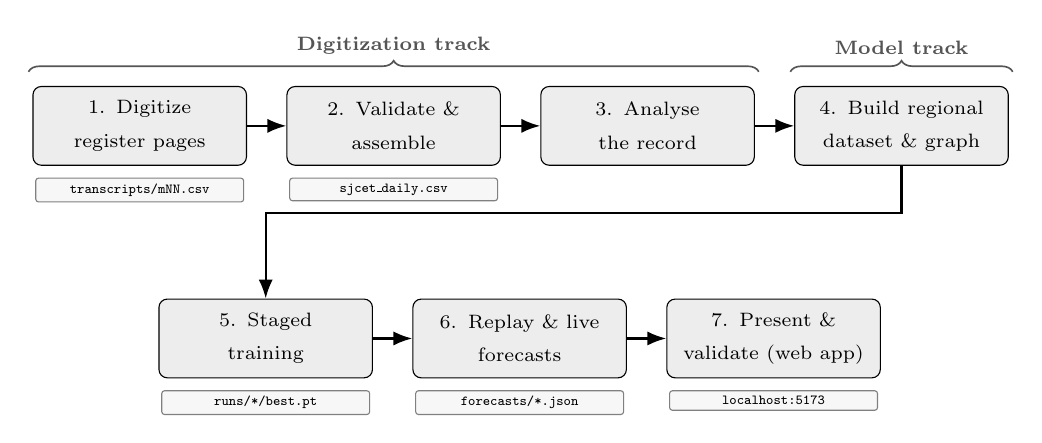
\begin{tikzpicture}[
        every node/.style={font=\scriptsize},
        wkstep/.style={draw=brandbrown, rounded corners=3pt, minimum width=2.7cm,
                       minimum height=1.0cm, fill=brandbeige, align=center,
                       text width=2.5cm, inner sep=3pt},
        file/.style={draw=brandrule, fill=brandcream, rounded corners=1pt, align=center,
                     font=\tiny\ttfamily, inner sep=2pt, text width=2.5cm},
        arrow/.style={-{Latex[length=2.4mm]}, brandbrown, line width=0.8pt},
        phase/.style={font=\scriptsize\bfseries, text=brandtan, align=center}
    ]
        \node[wkstep] (s1) at (0,0) {1. Digitize\\register pages};
        \node[wkstep, right=0.5cm of s1] (s2) {2. Validate \&\\assemble};
        \node[wkstep, right=0.5cm of s2] (s3) {3. Analyse\\the record};
        \node[wkstep, right=0.5cm of s3] (s4) {4. Build regional\\dataset \& graph};

        \node[wkstep] (s5) at (1.6,-2.7) {5. Staged\\training};
        \node[wkstep, right=0.5cm of s5] (s6) {6. Replay \& live\\forecasts};
        \node[wkstep, right=0.5cm of s6] (s7) {7. Present \&\\validate (web app)};

        \draw[arrow] (s1) -- (s2);
        \draw[arrow] (s2) -- (s3);
        \draw[arrow] (s3) -- (s4);
        \draw[arrow] (s4.south) -- ++(0,-0.6) -| (s5.north);
        \draw[arrow] (s5) -- (s6);
        \draw[arrow] (s6) -- (s7);

        \node[file, below=0.15cm of s1] {transcripts/mNN.csv};
        \node[file, below=0.15cm of s2] {sjcet\_daily.csv};
        \node[file, below=0.15cm of s5] {runs/*/best.pt};
        \node[file, below=0.15cm of s6] {forecasts/*.json};
        \node[file, below=0.15cm of s7] {localhost:5173};

        \draw[decorate, decoration={brace, amplitude=4pt}, brandtan, line width=0.6pt]
            ($(s1.north west)+(-0.05,0.18)$) -- ($(s3.north east)+(0.05,0.18)$);
        \node[phase, above=0.28cm] at ($(s1.north)!0.5!(s3.north)$) {Digitization track};
        \draw[decorate, decoration={brace, amplitude=4pt}, brandtan, line width=0.6pt]
            ($(s4.north west)+(-0.05,0.18)$) -- ($(s4.north east)+(0.05,0.18)$);
        \node[phase, above=0.28cm] at (s4.north) {Model track};
    \end{tikzpicture}
    \caption{\capFigPipeline}\label{fig:pipeline}
\end{figure}

\section{Data Sources}
\label{sec:sources}

\footnotesize
\begin{longtable}{|L{2.33cm}|L{5.02cm}|L{4.48cm}|}
\caption{\capTabSources}\label{tab:sources}\\
\hline
\textbf{Source} & \textbf{Content} & \textbf{Used for} \\
\hline
\endfirsthead
\hline
\textbf{Source} & \textbf{Content} & \textbf{Used for} \\
\hline
\endhead
SJCET weather register & Daily dry/wet bulb, max/min temperature and rainfall, Jul 2010 -- Dec 2016 (digitized by this work) & Stage-3 target; History page \\ \hline
NASA POWER & Daily MERRA-2-based reanalysis \cite{ref15}, 1990--2025: 1\textdegree{} over India, 0.5\textdegree{} over Kerala, plus a point at SJCET & Stage-1 pretraining; live inputs \\ \hline
NOAA GSOD \cite{ref12} & Daily station summaries: Bangalore, Coimbatore, Mangalore, Thiruvananthapuram, Kozhikode, Cochin & Stage-2 pretraining; live inputs \\ \hline
ERA5 (planned) & Hourly reanalysis aggregated to daily statistics & Not used: the Copernicus queue was too slow; downloader kept \\ \hline
\end{longtable}
\normalsize

\textbf{NASA POWER reanalysis.} The original plan used ERA5 daily statistics, but Copernicus requests sat in the queue for over an hour without starting. NASA POWER returns 36 years of daily data for one point in about four seconds without an API key, and was adopted instead; its resolution of about 0.5\textdegree{} set the resolution of the Kerala grid. Nine variables are taken for every grid node: daily maximum, minimum and mean 2-m temperature, 2-m dewpoint, precipitation, surface pressure, the $u$ and $v$ components of 10-m wind, and cloud amount. The India box spans 6--37\textdegree N, 68--98\textdegree E at 1\textdegree; the Kerala box spans 8--13\textdegree N, 74--78\textdegree E at 0.5\textdegree.

\textbf{NOAA GSOD stations.} Units are converted from \textdegree F and inches, incomplete precipitation totals are dropped, and basic range checks are applied (maximum 15--45\,\textdegree C, minimum 5--35\,\textdegree C, rain at most 500\,mm). Stations with less than 50\% coverage are excluded, leaving six.

\section{Digitization of the SJCET Register}
\label{sec:digitization}

The clean source is a scanned PDF with one page per month from July 2010 to December 2016 (78 months). A separate summary PDF gives the rainfall of each month and year, and a further 289 phone photographs cover later years and are not yet transcribed. Following the practice of historical data rescue \cite{ref1,ref2,ref3}, each page was processed as follows:

\begin{enumerate}
    \item \textbf{Transcribe} every cell exactly as written into one CSV per page, with a header giving the year, month and column order (two layouts occur, one up to 2011 and one from 2012).
    \item \textbf{Check} each page automatically: the row count matches the days in the month, values fall in physical ranges, the wet bulb does not exceed the dry bulb, the minimum is below the maximum, and the rain column sums to the written total.
    \item \textbf{Re-read} disagreements zoomed in, and decide whether the error is ours or the observer's.
    \item \textbf{Assemble} all pages onto a complete calendar, converting rain to millimetres, deriving relative humidity, and storing a flag and note for every row.
\end{enumerate}

A row is flagged \textbf{suspect} if its remarks describe a value as doubtful, unreadable or overwritten, if it breaks physics as written, if its rain may be accumulated over unobserved days, or if its month disagrees with the written total. The flag never deletes a value; it records the reason so that the modelling step can decide what to drop. Blank rain cells are stored as \textbf{not recorded}, never as zero.

\textbf{Rainfall checksums.} Together, the foot of the rain column (2014--2016) and the summary pages give a written total for every month. \textbf{59 of 78 months} match it to within 0.1\,cm. For six mismatched months a zoomed re-read confirmed the digits as transcribed, so these are addition errors by the observer; in the remaining months every rain value is kept but flagged.

\label{sec:dig-oddities}\textbf{Oddities.} The register has its own quirks: min/max headers swapped from 20 June 2011, dates written as ``-10'' in September 2011, ink bleed-through in June 2013, blank daily pages for November and December 2012 although the summary gives totals for both, and a maximum temperature that is often constant for weeks (for example 34\,\textdegree C every day of January 2013), which suggests the maximum thermometer was reset irregularly. The register yields 1,549 observed days in 2,376 calendar days (65\%), with weekends and holidays accounting for most gaps (Figure~\ref{fig:coverage}).

\begin{figure}[!htbp]
    \centering
    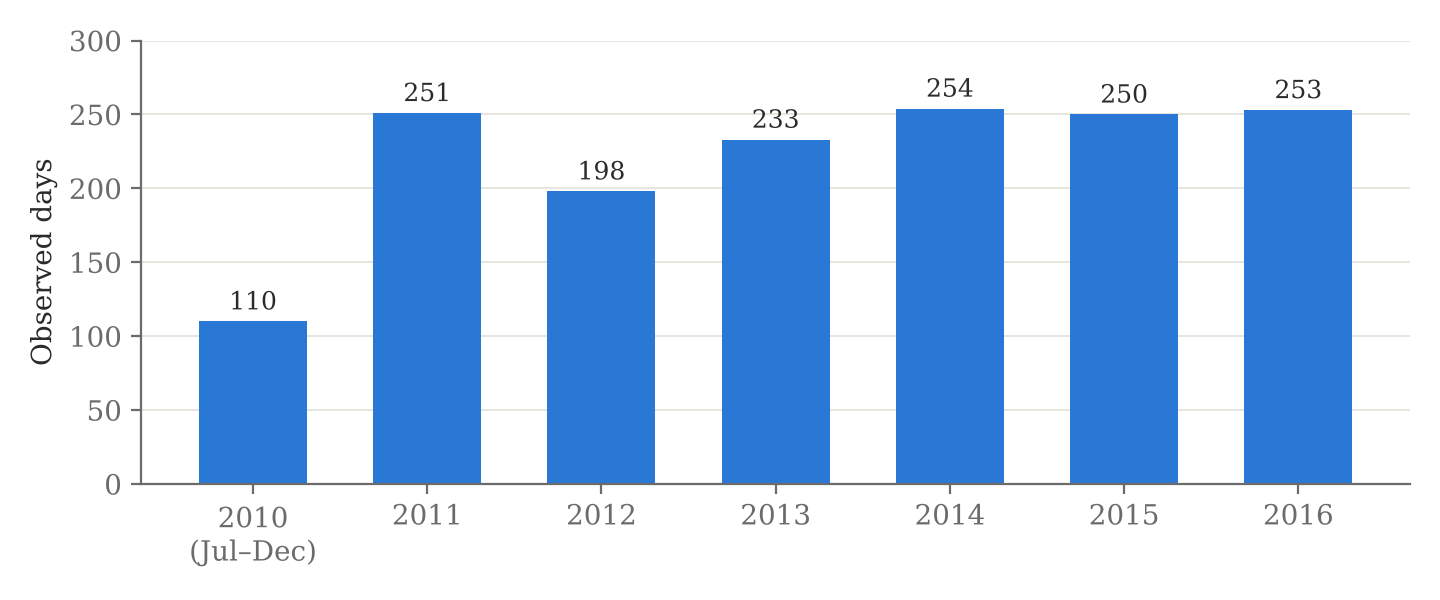
\includegraphics[width=0.85\textwidth]{register_coverage.png}
    \caption{\capFigCoverage}\label{fig:coverage}
\end{figure}

\label{sec:ocr}\textbf{Why not OCR.} The proposal planned an OCR route with table structure recognition \cite{ref2,ref4} and a handwriting recogniser. On 150 hand-labelled cells, zero-shot TrOCR \cite{ref11} read at best 35.3\% exactly (character error rate 0.48), and fine-tuning it needs a GPU the team did not have. For 78 months of pages, manual transcription with automatic checks was faster and more reliable, and, since table-recognition models depend on large labelled training sets \cite{ref10}, the transcripts now form a complete labelled set for training an OCR model \cite{ref3} on the later photographs.

\section{Preparing the Register for Modelling}
\label{sec:sjcet-handling}

The register is added to the graph as one station node, with four adjustments:

\begin{itemize}
    \item \textbf{08:30 reading convention.} Rain recorded on date $D$ fell between 08:30 on $D-1$ and 08:30 on $D$, and the maximum thermometer read on $D$ holds the maximum of $D-1$; both are moved to $D-1$, while the minimum stays on $D$.
    \item \textbf{Dewpoint} is computed from the 08:30 dry/wet-bulb pair (Equations~(\ref{eq:es})--(\ref{eq:td})); the daily mean is approximated as $(T_{\max}+T_{\min})/2$.
    \item \textbf{Suspect values} lose their rain value, and also their temperatures when the doubt concerns a reading rather than a monthly rain mismatch.
    \item \textbf{Accumulated rain.} A reading after an unread day contains several days of rain, so it is dropped rather than attributed to a single day.
\end{itemize}

With the dry-bulb temperature $T$ and the wet-bulb temperature $T_w$ in \textdegree C and a station pressure of about 1005\,hPa, the saturation vapour pressure, the actual vapour pressure and the dewpoint are
\begin{equation}
e_s(x)=6.112\,\exp\!\left(\frac{17.67\,x}{x+243.5}\right),
\label{eq:es}
\end{equation}
\begin{equation}
e=e_s(T_w)-0.000799\times1005\,(T-T_w),
\label{eq:e}
\end{equation}
\begin{equation}
T_d=\frac{243.5\,\ln(e/6.112)}{17.67-\ln(e/6.112)}.
\label{eq:td}
\end{equation}

After these steps the training period contains 716 SJCET temperature days and 249 rain days (July 2010 -- 2013); 2014 is used for validation and 2015--2016 for testing.

\section{Forecasting Model}
\label{sec:model}

\textbf{The weather graph.} Every source is assembled onto one daily calendar from 1990 to 2025 and every node is connected to its eight nearest neighbours by great-circle distance (Table~\ref{tab:graph}). Each edge carries the east--west and north--south offsets, the distance and the elevation difference. A graph \cite{ref7,ref13} accepts the coarse India grid, the fine Kerala grid, the irregular stations and SJCET as they are, without interpolation, and makes the transfer natural: SJCET is simply another node, hidden in stages 1 and 2 and revealed in stage 3.

\begin{table}[!htbp]
    \centering
    \caption{\capTabGraph}\label{tab:graph}
    \footnotesize
    \begin{tabularx}{\textwidth}{|L{4.4cm}|C{1.6cm}|Y|}
        \hline
        \textbf{Node group} & \textbf{Count} & \textbf{Notes} \\ \hline
        Reanalysis, India 1\textdegree & 962 & Coarse context; loss weight 0.1 in stage 2 \\ \hline
        Reanalysis, Kerala 0.5\textdegree & 99 & Fine grid around the target \\ \hline
        Reanalysis point at SJCET & 1 & Reanalysis value at the campus location \\ \hline
        NOAA GSOD stations & 6 & Real observations; loss weight 2 in stage 2 \\ \hline
        SJCET register & 1 & Hidden in stages 1--2; the only loss node in stage 3 \\ \hline
        \textbf{Total} & \textbf{1,069} & $k=8$ nearest neighbours, symmetrised \\ \hline
    \end{tabularx}
\end{table}

\textbf{Inputs and outputs.} Table~\ref{tab:io} lists what each node sees and predicts. Each variable is normalised with statistics from the stage-1 training years on reanalysis nodes,
\begin{equation}
\tilde{x}_{v,t,k}=\frac{g_k(x_{v,t,k})-\mu_k}{\sigma_k}, \qquad g_k(x)=\begin{cases}\log(1+x) & k=\text{rain}\\ x & \text{otherwise}\end{cases}
\label{eq:norm}
\end{equation}
and missing values are set to zero and flagged by a separate mask channel, so the model learns the difference between ``zero'' and ``unknown''. This matters because SJCET is missing on every weekend and holiday. Relative humidity is derived from the forecast mean temperature $T$ and dewpoint $T_d$,
\begin{equation}
\mathrm{RH}=100\,\frac{E(T_d)}{E(T)}, \qquad E(x)=6.112\,\exp\!\left(\frac{17.62\,x}{243.12+x}\right).
\label{eq:rh}
\end{equation}

\begin{table}[!htbp]
    \centering
    \caption{\capTabIO}\label{tab:io}
    \footnotesize
    \begin{tabularx}{\textwidth}{|L{2.6cm}|Y|}
        \hline
        \textbf{Inputs} & Last 7 days of 9 variables (tmax, tmin, tmean, dewpoint, rain, surface pressure, $u_{10}$, $v_{10}$, cloud), normalised; the matching 7$\times$9 missing-value mask; latitude, longitude, elevation, node type (reanalysis/station); and the day of year of the first forecast day as $(\sin,\cos)$. \\ \hline
        \textbf{Outputs} & For each lead day $d=1,\dots,6$: tmax, tmin, rain ($\log(1+x)$), tmean, dewpoint, and a logit for rain $\geq$ 2.5\,mm (the IMD rainy-day threshold). \\ \hline
        \textbf{Derived} & Relative humidity, from the forecast tmean and dewpoint with the Magnus formula; it is not predicted directly. \\ \hline
    \end{tabularx}
\end{table}

\textbf{Network.} \textbf{WeatherGNN} follows the encode--process--decode pattern of graph-based weather models (Figure~\ref{fig:gnn}). A two-layer MLP encodes each node into a 128-dimensional state; four processor blocks each apply layer normalisation, a GATv2 convolution \cite{ref13} with four heads and edge features, and a feed-forward block, both with residual connections; and an MLP decoder emits all six lead days at once, which avoids error accumulation. The model has about 0.4\,M parameters and trains on a CPU. Each processor block updates the hidden state $h_i$ of node $i$ as
\begin{align}
h_i &\leftarrow h_i + \mathrm{Drop}\big(\mathrm{GATv2}(\mathrm{LN}(h))_i\big), \label{eq:block1}\\
h_i &\leftarrow h_i + \mathrm{Drop}\big(\mathrm{FFN}(h_i)\big), \label{eq:block2}
\end{align}
where the GATv2 layer \cite{ref13} aggregates the neighbours $j\in\mathcal{N}(i)$ with attention weights computed from both node states and the edge features $e_{ij}$:
\begin{equation}
\alpha_{ij}=\operatorname*{softmax}_{j\in\mathcal{N}(i)}\Big(a^{\top}\,\mathrm{LeakyReLU}\big(\Theta_s h_i+\Theta_t h_j+\Theta_e e_{ij}\big)\Big), \qquad
\mathrm{GATv2}(h)_i=\sum_{j\in\mathcal{N}(i)}\alpha_{ij}\,\Theta_t h_j .
\label{eq:gat}
\end{equation}

\begin{figure}[!htbp]
    \centering
    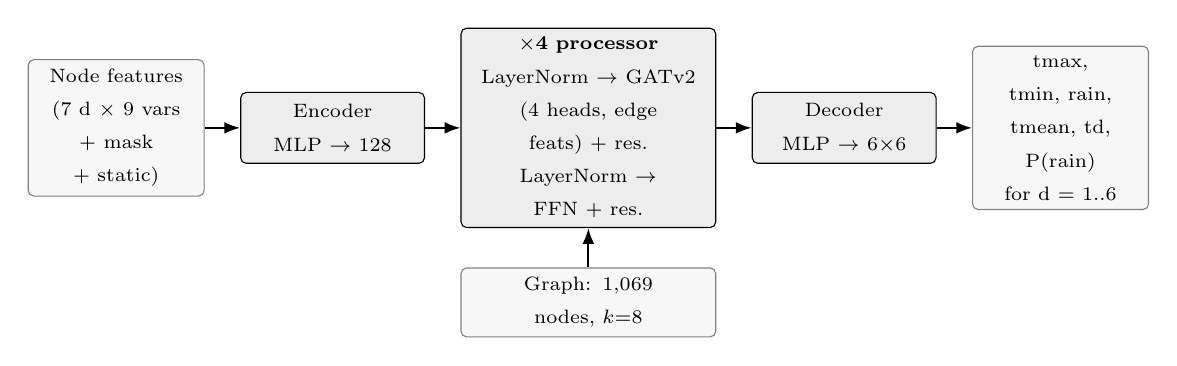
\begin{tikzpicture}[
        every node/.style={font=\scriptsize},
        blk/.style={draw=brandbrown, rounded corners=2pt, fill=brandbeige, align=center, minimum height=0.9cm, text width=2.1cm},
        io/.style={draw=brandrule, rounded corners=2pt, fill=brandcream, align=center, minimum height=0.9cm, text width=2.0cm},
        arrow/.style={-{Latex[length=2mm]}, brandbrown, line width=0.8pt}
    ]
        \node[io] (x) at (0,0) {Node features\\(7 d $\times$ 9 vars\\+ mask + static)};
        \node[blk, right=0.45cm of x] (enc) {Encoder\\MLP $\to$\allowbreak{} 128};
        \node[blk, right=0.45cm of enc, text width=3.0cm, minimum height=1.6cm] (proc) {\textbf{$\times$4 processor}\\LayerNorm $\to$\allowbreak{} GATv2\\(4 heads, edge feats) + res.\\LayerNorm $\to$\allowbreak{} FFN + res.};
        \node[blk, right=0.45cm of proc] (dec) {Decoder\\MLP $\to$\allowbreak{} 6$\times$6};
        \node[io, right=0.45cm of dec] (y) {tmax, tmin, rain,\\tmean, td, P(rain)\\for d = 1..6};
        \draw[arrow] (x) -- (enc); \draw[arrow] (enc) -- (proc); \draw[arrow] (proc) -- (dec); \draw[arrow] (dec) -- (y);
        \node[io, below=0.5cm of proc, text width=3.0cm, minimum height=0.6cm] (g) {Graph: 1,069 nodes, $k$=8};
        \draw[arrow] (g) -- (proc);
    \end{tikzpicture}
    \caption{\capFigGnn}\label{fig:gnn}
\end{figure}

\textbf{Loss.} The loss is a masked, node-weighted mean squared error over the regression targets plus half a weighted binary cross-entropy for rain occurrence,
\begin{equation}
\mathcal{L} = \frac{\sum m\,w\,(\hat{y}-y)^2}{\sum m\,w} \;+\; 0.5\,\frac{\sum m\,w\,\mathrm{BCE}_{p^{+}=2}(\hat{z},o)}{\sum m\,w},
\label{eq:loss}
\end{equation}
where $m$ is the target mask, $w$ the per-node stage weight, $\hat{z}$ the rain logit and $o$ the observed occurrence. A missing target contributes nothing.

\section{Staged Transfer Learning}
\label{sec:stages}

Each stage of the transfer \cite{ref7,ref8} closes a different gap (Figure~\ref{fig:method}, Table~\ref{tab:stages}). Stage 1 learns \textbf{weather}: how the nine variables evolve over seven days across India. Stage 2 learns the \textbf{observation gap}: how real thermometers and rain gauges differ from reanalysis in the region. Stage 3 learns \textbf{SJCET}: its 08:30 convention, its whole-degree readings and its slope location. The splits are identical in every stage, and the checkpoint with the lowest validation loss is kept.

\begin{figure}[!htbp]
    \centering
    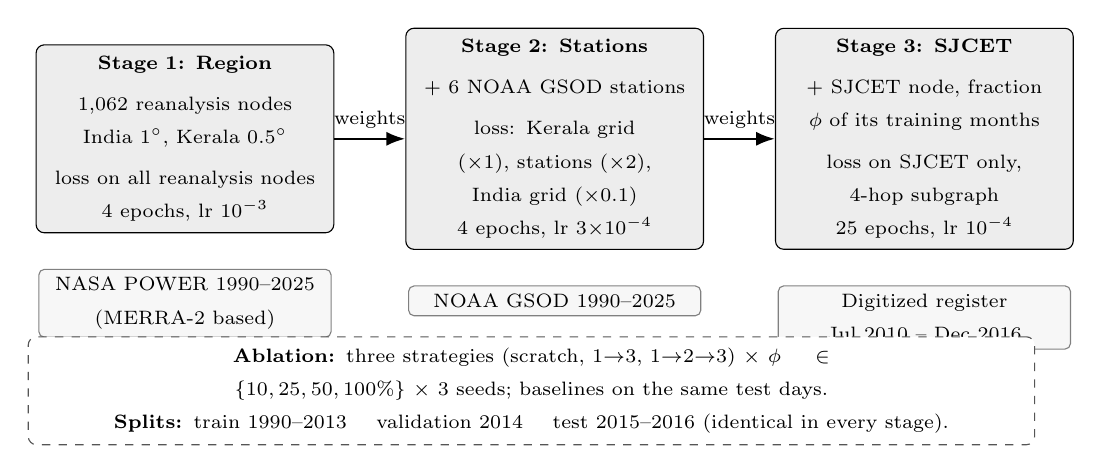
\begin{tikzpicture}[
        every node/.style={font=\scriptsize},
        box/.style={draw=brandbrown, rounded corners=3pt, fill=brandbeige, align=center,
                    text width=3.5cm, minimum height=2.3cm, inner sep=4pt},
        src/.style={draw=brandrule, rounded corners=2pt, fill=brandcream, align=center,
                    text width=3.5cm, inner sep=3pt},
        arrow/.style={-{Latex[length=2.4mm]}, brandbrown, line width=0.9pt},
    ]
        \node[box] (b1) at (0,0) {\textbf{Stage 1: Region}\\[1mm] 1,062 reanalysis nodes\\ India 1\textdegree, Kerala 0.5\textdegree\\[1mm] loss on all reanalysis nodes\\ 4 epochs, lr $10^{-3}$};
        \node[box, right=0.9cm of b1] (b2) {\textbf{Stage 2: Stations}\\[1mm] + 6 NOAA GSOD stations\\[1mm] loss: Kerala grid ($\times$1), stations ($\times$2), India grid ($\times$0.1)\\ 4 epochs, lr $3{\times}10^{-4}$};
        \node[box, right=0.9cm of b2] (b3) {\textbf{Stage 3: SJCET}\\[1mm] + SJCET node, fraction $\phi$ of its training months\\[1mm] loss on SJCET only, 4-hop subgraph\\ 25 epochs, lr $10^{-4}$};
        \draw[arrow] (b1) -- node[above]{weights} (b2);
        \draw[arrow] (b2) -- node[above]{weights} (b3);
        \node[src, below=0.45cm of b1] {NASA POWER 1990--2025\\(MERRA-2 based)};
        \node[src, below=0.45cm of b2] {NOAA GSOD 1990--2025};
        \node[src, below=0.45cm of b3] {Digitized register\\Jul 2010 -- Dec 2016};
        \node[draw=brandtan, dashed, rounded corners=3pt, fill=white, text width=12.5cm, align=center, inner sep=4pt]
            at (4.4,-3.2) {\textbf{Ablation:} three strategies (scratch, 1$\to$\allowbreak{}3, 1$\to$\allowbreak{}2$\to$\allowbreak{}3) $\times$ $\phi\in\{10,25,50,100\%\}$ $\times$ 3 seeds; baselines on the same test days.\\
            \textbf{Splits:} train 1990--2013 \quad validation 2014 \quad test 2015--2016 (identical in every stage).};
    \end{tikzpicture}
    \caption{\capFigMethod}\label{fig:method}
\end{figure}

\begin{table}[!htbp]
    \centering
    \caption{\capTabStages}\label{tab:stages}
    \footnotesize
    \begin{tabularx}{\textwidth}{|C{1.1cm}|L{4.2cm}|Y|}
        \hline
        \textbf{Stage} & \textbf{Data the model sees} & \textbf{Loss on} \\ \hline
        1 & Reanalysis nodes only & All reanalysis nodes (weight 1) \\ \hline
        2 & + NOAA stations (SJCET still hidden) & Kerala 0.5\textdegree{} nodes (1), stations (2), India 1\textdegree{} nodes (0.1) \\ \hline
        3 & + SJCET, a fraction $\phi$ of its training months & SJCET only, on its 4-hop subgraph \\ \hline
    \end{tabularx}
\end{table}

Because the network has four message-passing layers, only nodes within four hops of SJCET can influence its output, so stage 3 runs on that subgraph alone. The fraction $\phi$ is applied to whole months, shuffled with the run's seed, so a 10\% run sees a few complete months rather than scattered days. Table~\ref{tab:hyper} gives the training settings.

\begin{table}[!htbp]
    \centering
    \caption{\capTabHyper}\label{tab:hyper}
    \footnotesize
    \begin{tabularx}{\textwidth}{|L{4.6cm}|Y|}
        \hline
        \textbf{Setting} & \textbf{Value} \\ \hline
        Input window / horizon & 7 days / 6 lead days \\ \hline
        Hidden size, layers, heads, dropout & 128, 4, 4, 0.1 \\ \hline
        Optimiser & AdamW, weight decay $10^{-4}$, gradient clipping at 1.0 \\ \hline
        Schedule & One-cycle learning rate, 10\% warm-up \\ \hline
        Epochs / learning rate & Stage 1: 4 / $10^{-3}$ (continued from a one-day-horizon model); stage 2: 4 / $3{\times}10^{-4}$; stage 3: 25 / $10^{-4}$ (pretrained) or $10^{-3}$ (scratch) \\ \hline
        Batch / steps per epoch & 16 random days / up to 150 batches \\ \hline
        Early stopping & Patience 4 epochs on validation loss; best checkpoint kept \\ \hline
        Seeds & 0, 1, 2 for fractions below 100\%; seed 0 at 100\% \\ \hline
    \end{tabularx}
\end{table}

\label{sec:method-missing}\textbf{Missing data.} A seven-day input window at SJCET usually has two or more missing days. Inputs are handled by the mask channel and targets by masking the loss. An optional variant (\textbf{-{}-clim-fill}) feeds a smoothed day-of-year climatology of SJCET in place of missing inputs while keeping the mask set to ``missing''.

\label{sec:live}\textbf{Live forecasting.} \textbf{live.py} fetches recent NASA POWER data for SJCET's 4-hop neighbourhood and the latest GSOD files, builds the seven-day window ending on the last complete day, and runs the default region$\to$\allowbreak{}stations$\to$\allowbreak{}SJCET model. NASA POWER publishes about three days late, so today is usually lead day 4, which is why the horizon was extended to six days. Because the register stops in 2016, SJCET's own inputs are empty in a live forecast; a live-like test (Section~\ref{sec:res-livelike}) measures the effect.

\section{Evaluation Setup}
\label{sec:evaluation}

Four baselines, including XGBoost \cite{ref14}, are scored on exactly the same SJCET test days and, where they use training data, the same subset of training months as the GNN they are compared with (Table~\ref{tab:baselines}).

\begin{table}[!htbp]
    \centering
    \caption{\capTabBaselines}\label{tab:baselines}
    \footnotesize
    \begin{tabularx}{\textwidth}{|L{2.6cm}|Y|}
        \hline
        \textbf{Baseline} & \textbf{Definition} \\ \hline
        Persistence & Every lead day equals today's SJCET observation (``tomorrow = today''). Scored only on days that follow a reading. \\ \hline
        Climatology & Day-of-year mean of SJCET's training months, smoothed over $\pm$15 days. \\ \hline
        Reanalysis & NASA POWER value at the nearest grid node on the target day. It is not a forecast; it shows how far gridded reanalysis is from the station even with perfect knowledge of the day. \\ \hline
        XGBoost \cite{ref14} & SJCET's last 7 days of five variables plus the nearest grid node's last 7 days of nine variables plus the day of year; one model per lead day and target (300 trees, depth 5, learning rate 0.05). \\ \hline
        GNN from scratch & The same network and stage-3 procedure with random initial weights, serving as the control for pretraining. \\ \hline
    \end{tabularx}
\end{table}

For $n$ test days with forecasts $\hat{y}_i$ and observations $y_i$ the main scores are
\begin{equation}
\mathrm{RMSE}=\sqrt{\frac{1}{n}\sum_{i=1}^{n}(\hat{y}_i-y_i)^2}, \qquad \mathrm{MAE}=\frac{1}{n}\sum_{i=1}^{n}\lvert\hat{y}_i-y_i\rvert,
\label{eq:rmse}
\end{equation}
\begin{equation}
\mathrm{Bias}=\frac{1}{n}\sum_{i=1}^{n}(\hat{y}_i-y_i), \qquad R^2=1-\frac{\sum_i(\hat{y}_i-y_i)^2}{\sum_i(y_i-\bar{y})^2},
\label{eq:bias}
\end{equation}
and, for the rain probability $p_i$ and observed occurrence $o_i\in\{0,1\}$, the Brier score is $\frac{1}{n}\sum_i(p_i-o_i)^2$. Forecast \textbf{accuracy}, the primary result, is reported as $100-\mathrm{MAPE}$ for temperature together with the share of forecasts within $\pm$1 and $\pm$2\,\textdegree C of the register reading; rain occurrence ($\geq$2.5\,mm) is scored by rain/no-rain accuracy, hit rate and false-alarm ratio. All metrics are computed in physical units at the SJCET node, separately for each lead day. Four experiments are run: a \textbf{full-data comparison} with all SJCET training months; a \textbf{data-efficiency ablation} over three strategies, four fractions and three seeds; a \textbf{live-like test} with SJCET's own inputs hidden; and a \textbf{seasonal breakdown} of the day-1 error.

\setcounter{equation}{0}
\chapter{Results and Discussion}
\label{chap:results}

This chapter presents the outcomes of Phase 1 of the project. The phase covered the digitization of the SJCET register, the construction of the regional dataset, the three-stage training of the forecasting model, its evaluation against conventional baselines, and the web application that presents the forecasts. All scores are computed at the SJCET node over the 2015--2016 test period, on every day for which the register has a reading.

\section{Dataset Preparation and Preprocessing Results}
\label{sec:res-data}

The digitization of the July 2010 -- December 2016 register produced a daily dataset of \textbf{1,549 observed days} out of 2,376 calendar days, with weekends and holidays accounting for most of the gaps (Figure~\ref{fig:coverage}). Every value is traceable to its page, and \textbf{59 of the 78 months} agree with the observers' own written rainfall totals to within 0.1\,cm. For six of the mismatched months a zoomed re-read showed the transcription to be correct and the error to be the observer's addition. Overall, 1,095 days are flagged \textbf{ok} and 454 \textbf{suspect}, mostly because of a monthly rain-total mismatch that casts doubt on the rain values rather than the temperatures.

The register is unusual as a training target. It is read only on weekdays, it records most temperatures in whole degrees, its rain gauge is emptied only when read, and its maximum thermometer often shows the same value for weeks. After the 08:30 reading convention is applied and accumulated or doubtful values are removed, the training period contains \textbf{716 temperature days} and only \textbf{249 rain days}.

The regional dataset joins 36 years (1990--2025) of NASA POWER reanalysis at 1,062 grid points, six NOAA stations and the SJCET node into a single graph of \textbf{1,069 nodes and 8,884 edges} (Figure~\ref{fig:graphmap}). It provides 8,754 training days for stages 1 and 2, against 1,194 candidate days for stage 3 at SJCET.

\begin{figure}[!htbp]
    \centering
    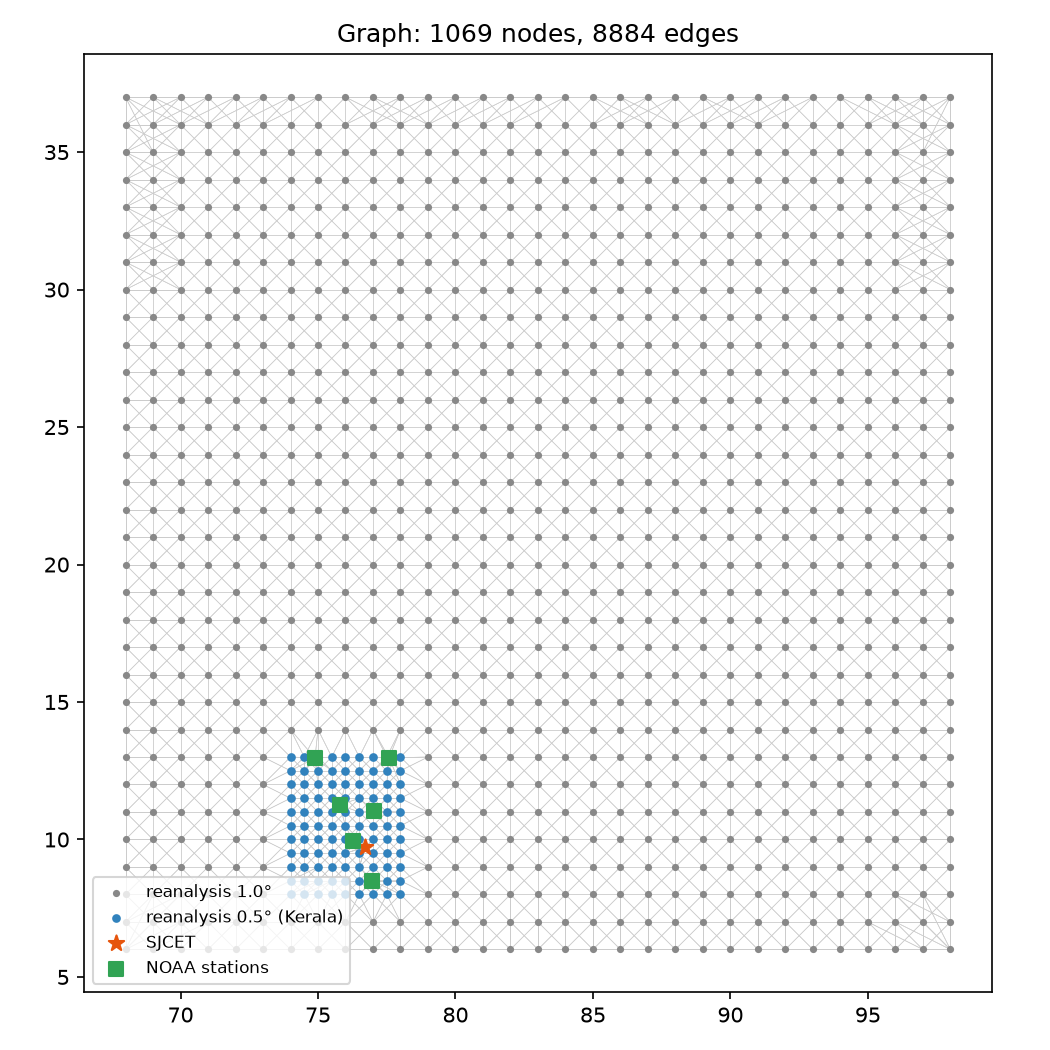
\includegraphics[width=0.62\textwidth]{graph_map.png}
    \caption{\capFigGraphMap}\label{fig:graphmap}
\end{figure}

\section{Training Progress}
\label{sec:res-training}

The model was trained in three stages on a CPU. Stage 1, first trained at a one-day horizon, was continued for 4 epochs at the six-day horizon; its validation loss fell from 0.357 to 0.344, at about 400 seconds per epoch over the full 1,069-node graph. Stage 2 ran for a further 4 epochs and its validation loss fell from 0.385 to 0.379. Stage 3 trains on SJCET's 4-hop subgraph only, so each epoch takes about 12 seconds. The pretrained models reached their lowest validation loss after 2 epochs (0.722 for 1$\to$\allowbreak{}2$\to$\allowbreak{}3) and early stopping ended training after 6, while the network trained from scratch needed 5 epochs and fluctuated much more between epochs. A pretrained network therefore needs very little local training to adapt.

The results are reproducible. For this report the evaluation was re-run on a separate machine (\textbf{train.py -{}-eval-only}) and reproduced every score to two decimal places, and the main stage-3 model was retrained from the stage-2 checkpoint (\textbf{train.py -{}-stage 3 -{}-init s12/\allowbreak{}best.pt -{}-fraction 1.0 -{}-seed 0}) and matched the original training log at every epoch.

\section{Forecast Accuracy}
\label{sec:res-accuracy}

Forecast accuracy is the headline result of the project. For temperature it is measured as $100-\mathrm{MAPE}$, the percentage by which a forecast agrees with the register reading, and for rain as the percentage of days on which the forecast correctly says whether it rains ($\geq$2.5\,mm). Table~\ref{tab:accuracy} gives both for every model, one and six days ahead, and Figure~\ref{fig:timeseries} compares the next-day forecasts of the final model with the register over the whole test period.

\begin{table}[!htbp]
    \centering
    \caption{\capTabAccuracy}\label{tab:accuracy}
    \footnotesize
    \begin{tabularx}{\textwidth}{|L{4.6cm}|C{1.45cm}|C{1.45cm}|C{1.45cm}|C{1.45cm}|Y|}
        \hline
        \textbf{Model} & \textbf{Tmax d1 (\%)} & \textbf{Tmin d1 (\%)} & \textbf{Tmax d6 (\%)} & \textbf{Tmin d6 (\%)} & \textbf{Rain/no-rain d1 (\%)} \\ \hline
        GNN 1$\to$\allowbreak{}2$\to$\allowbreak{}3 (region$\to$\allowbreak{}stations$\to$\allowbreak{}SJCET) & 96.6 & 96.2 & 96.3 & 95.8 & 64.0 \\ \hline
        GNN 1$\to$\allowbreak{}3 (region$\to$\allowbreak{}SJCET) & 96.7 & 96.1 & \textbf{96.4} & 95.6 & 63.3 \\ \hline
        GNN from scratch (SJCET only) & 94.9 & 94.1 & 95.7 & 94.8 & 63.3 \\ \hline
        GNN stage 1 only (no SJCET data) & 91.0 & 91.3 & 89.9 & 92.0 & 73.8 \\ \hline
        GNN stages 1$\to$\allowbreak{}2 (no SJCET data) & 90.9 & 91.6 & 90.1 & 92.5 & 73.5 \\ \hline
        XGBoost (station + nearest grid) & 96.6 & 96.4 & 96.1 & 95.6 & 53.8 \\ \hline
        Climatology & 95.3 & 95.7 & 95.4 & 95.7 & 50.9 \\ \hline
        Persistence & \textbf{97.8} & \textbf{97.8} & \textbf{96.4} & \textbf{96.0} & 75.3 \\ \hline
        Reanalysis at nearest grid node & 87.8 & 94.7 & 87.8 & 94.7 & \textbf{77.5} \\ \hline
    \end{tabularx}
\end{table}

\begin{figure}[!htbp]
    \centering
    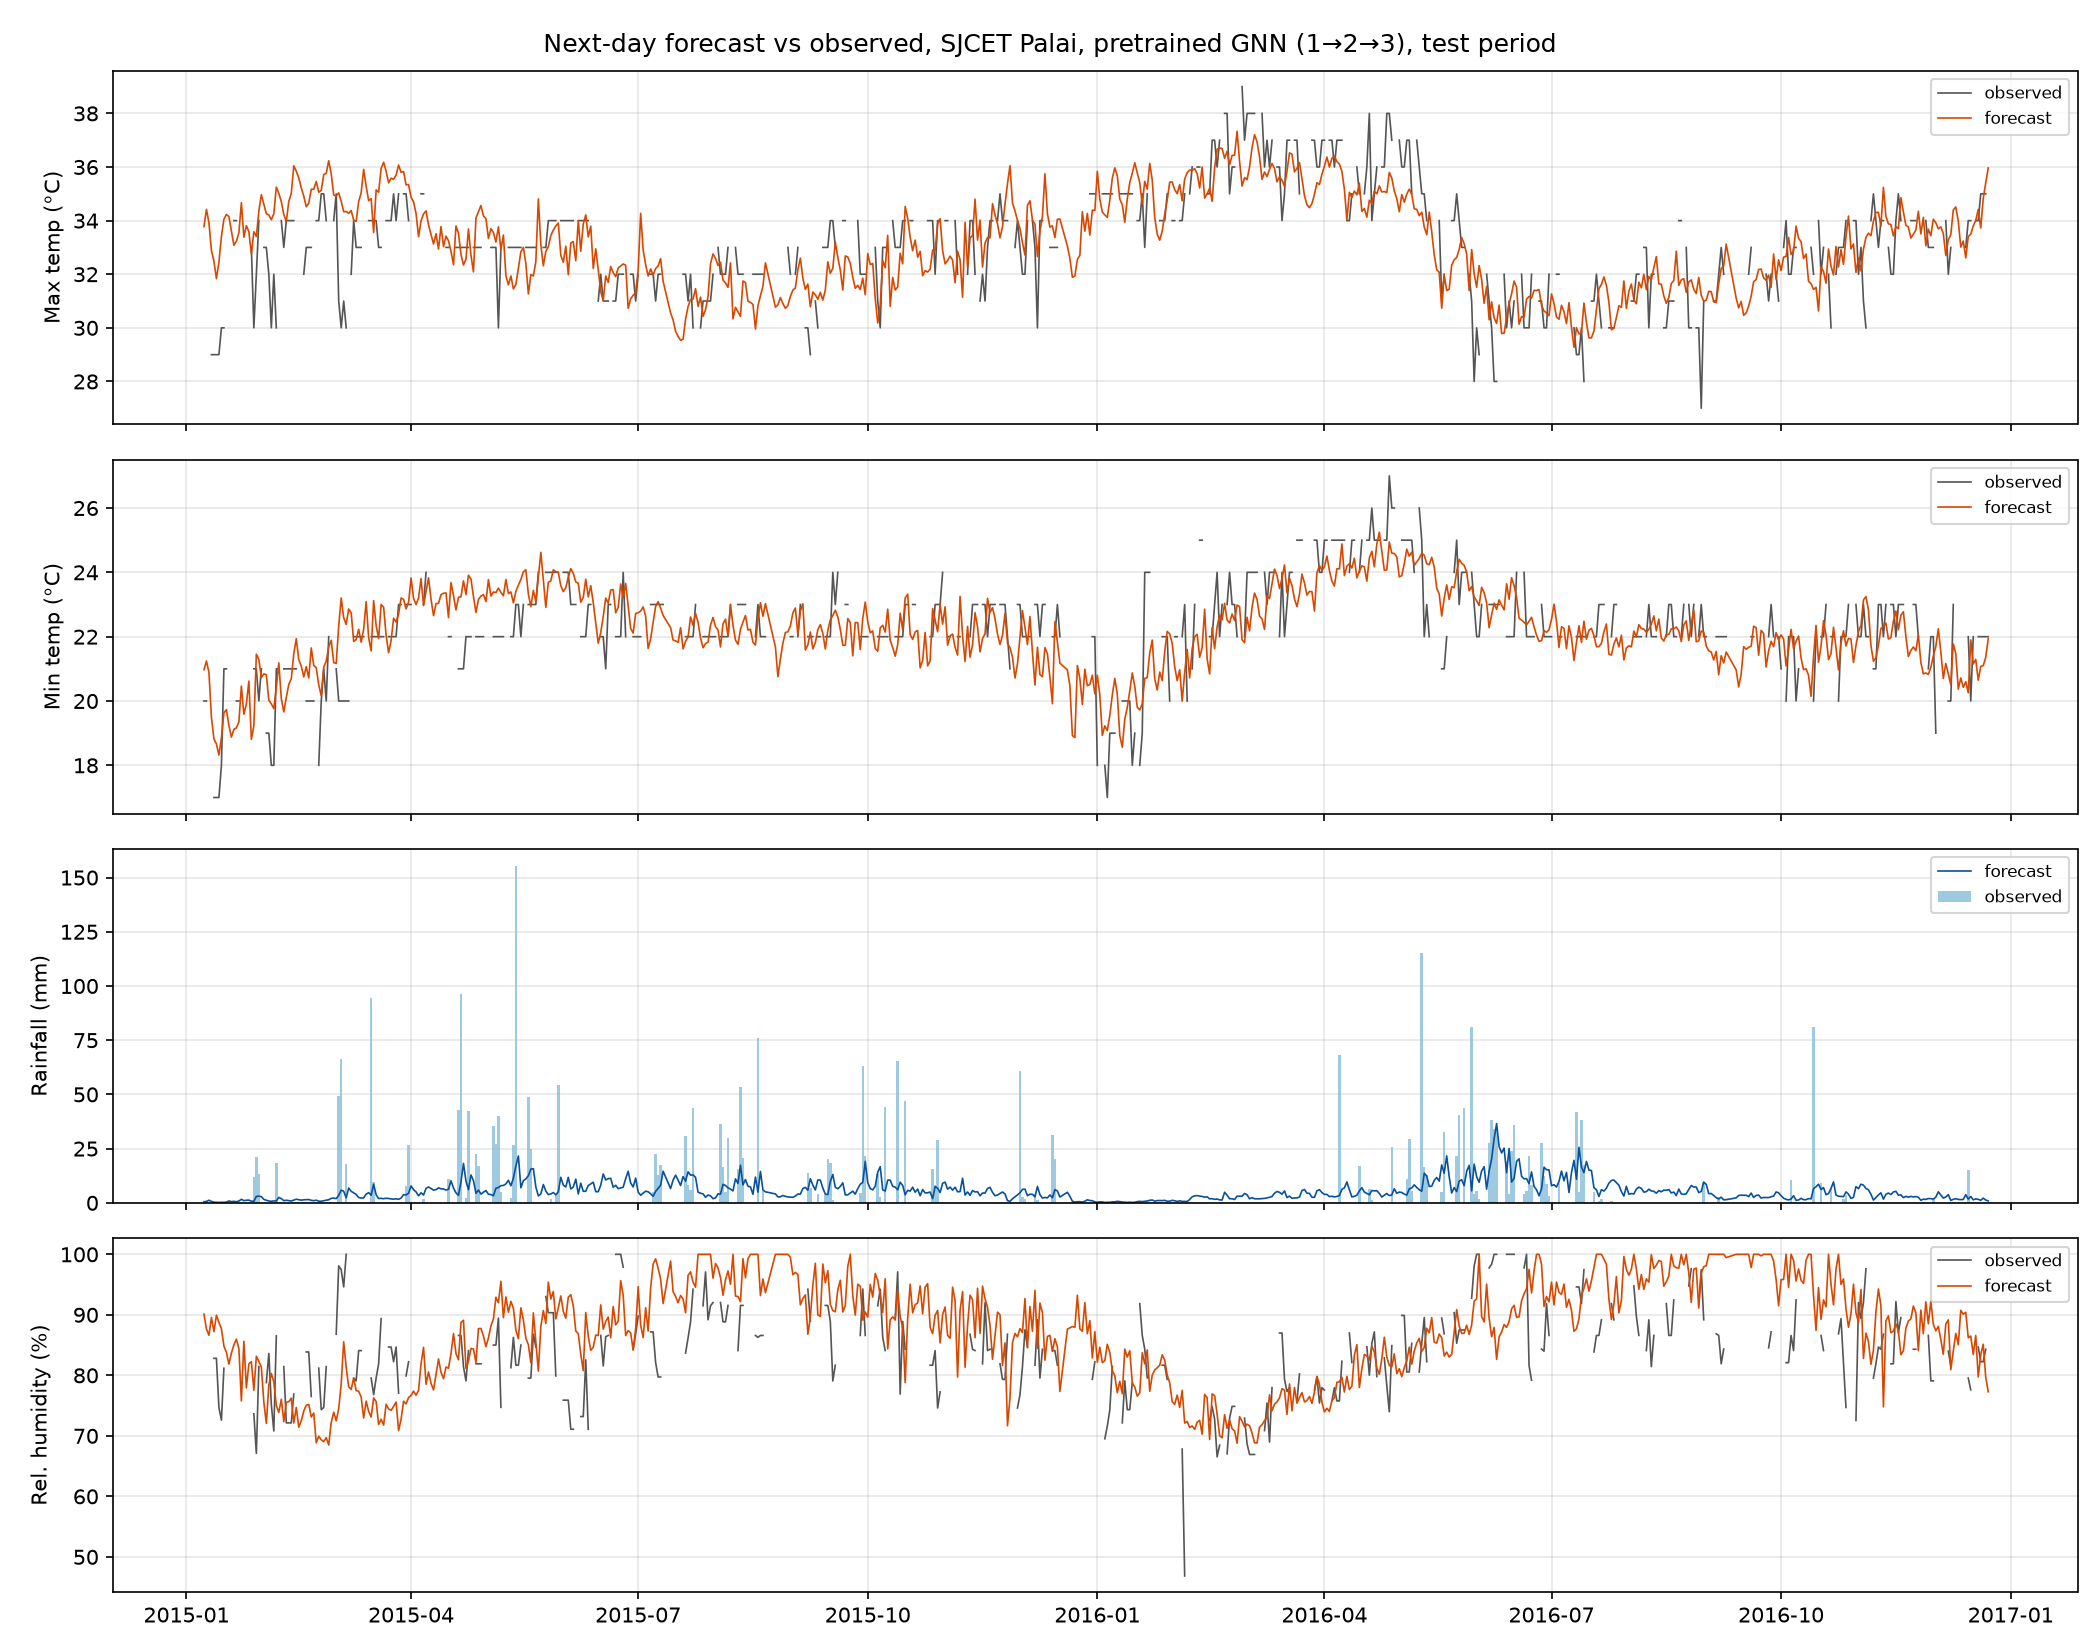
\includegraphics[width=0.95\textwidth]{test_timeseries.png}
    \caption{\capFigTimeseries}\label{fig:timeseries}
\end{figure}

\begin{itemize}
    \item \textbf{The final model forecasts temperature with about 96\% accuracy.} The region$\to$\allowbreak{}stations$\to$\allowbreak{}SJCET model forecasts the next day's maximum temperature with \textbf{96.6\%} accuracy and the minimum with \textbf{96.2\%}. In practical terms, \textbf{86\%} of its maximum-temperature forecasts and \textbf{93\%} of its minimum-temperature forecasts fall within $\pm$2\,\textdegree C of the register reading (55\% and 65\% within $\pm$1\,\textdegree C). Accuracy stays above 95.7\% six days ahead.
    \item \textbf{Pretraining is what delivers this accuracy.} The same network trained only on SJCET reaches 94.9\% and 94.1\%, with only 62\% of maximum-temperature forecasts within $\pm$2\,\textdegree C. Models that never see SJCET reach only about 91\%.
    \item \textbf{Against the baselines}, the pretrained GNNs are level with XGBoost and ahead of climatology. Persistence is the most accurate one day ahead (97.8\%), because the register repeats whole-degree values for days at a time, but by day 6 it falls to the level of the pretrained GNNs.
    \item \textbf{Rain is the weakest variable.} The fine-tuned GNNs call rain or no rain correctly on 63--64\% of days, below persistence (75\%) and the raw reanalysis (78\%).
\end{itemize}

\section{Error Comparison with Baselines}
\label{sec:res-full}

Table~\ref{tab:results} gives the same comparison as root-mean-square error (RMSE), and Figure~\ref{fig:rmse} shows it at every lead day.

\begin{table}[!htbp]
    \centering
    \caption{\capTabResults}\label{tab:results}
    \footnotesize
    \begin{tabularx}{\textwidth}{|L{3.9cm}|C{1.2cm}|C{1.2cm}|C{1.2cm}|C{1.45cm}|C{1.2cm}|Y|}
        \hline
        \textbf{Model} & \textbf{Tmax d1 (\textdegree C)} & \textbf{Tmin d1 (\textdegree C)} & \textbf{Rain d1 (mm)} & \textbf{Rain occ.\ acc.\ d1} & \textbf{Tmax d6 (\textdegree C)} & \textbf{Tmin d6 (\textdegree C)} \\ \hline
        GNN 1$\to$\allowbreak{}2$\to$\allowbreak{}3 (region$\to$\allowbreak{}stations$\to$\allowbreak{}SJCET) & 1.43 & 1.08 & 20.7 & 0.64 & 1.58 & \textbf{1.21} \\ \hline
        GNN 1$\to$\allowbreak{}3 (region$\to$\allowbreak{}SJCET) & 1.42 & 1.10 & 20.9 & 0.63 & \textbf{1.55} & 1.25 \\ \hline
        GNN from scratch (SJCET only) & 2.17 & 1.72 & 20.8 & 0.63 & 1.85 & 1.43 \\ \hline
        GNN stage 1 only (no SJCET data) & 3.40 & 2.16 & 22.6 & 0.74 & 3.75 & 2.04 \\ \hline
        GNN stages 1$\to$\allowbreak{}2 (no SJCET data) & 3.46 & 2.13 & 22.3 & 0.74 & 3.71 & 1.96 \\ \hline
        XGBoost (station + nearest grid) & 1.48 & 1.04 & 21.4 & 0.54 & 1.67 & 1.26 \\ \hline
        Climatology & 1.92 & 1.24 & 21.4 & 0.51 & 1.89 & 1.23 \\ \hline
        Persistence & \textbf{1.12} & \textbf{0.90} & 30.1 & 0.75 & 1.71 & 1.33 \\ \hline
        Reanalysis at nearest grid node & 4.55 & 1.58 & \textbf{20.5} & \textbf{0.78} & 4.56 & 1.59 \\ \hline
    \end{tabularx}
\end{table}

\begin{figure}[!htbp]
    \centering
    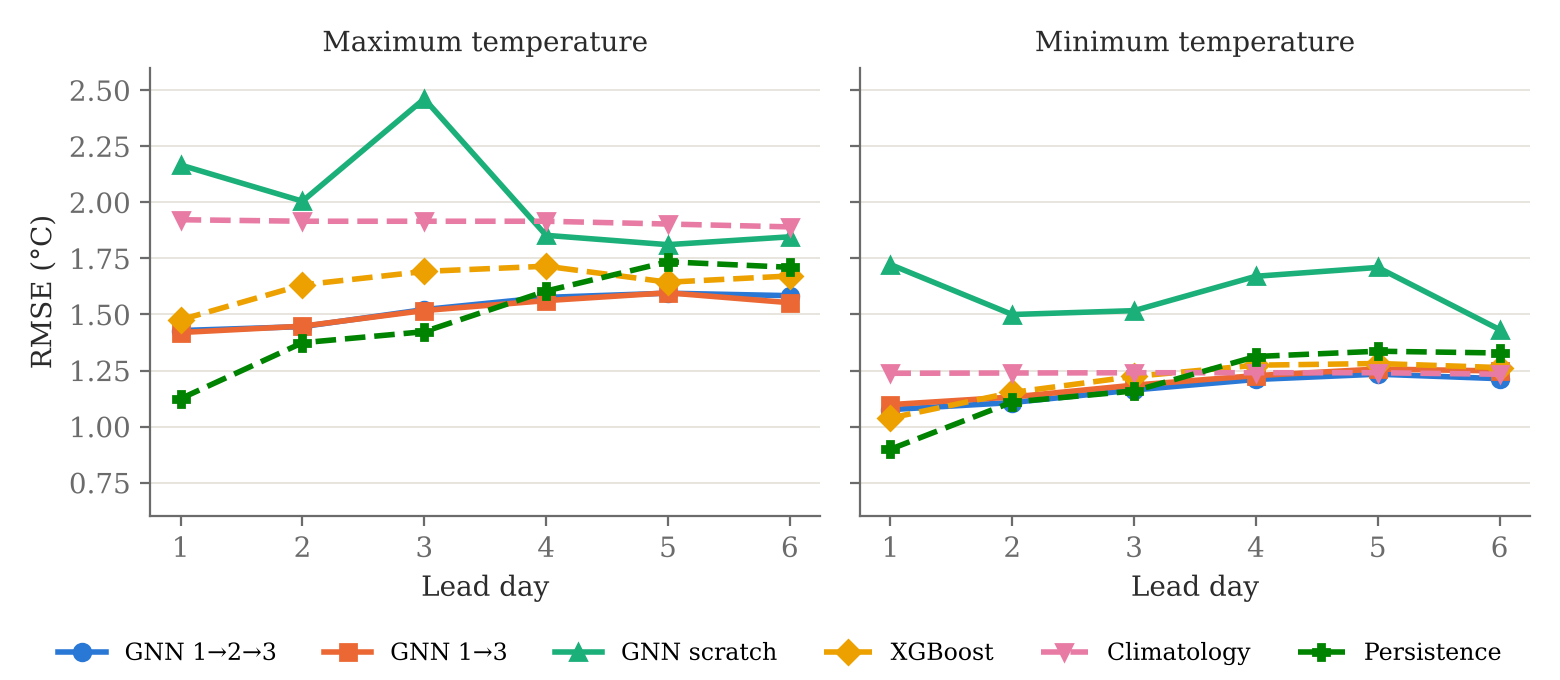
\includegraphics[width=0.98\textwidth]{rmse_lead.png}
    \caption{\capFigRmse}\label{fig:rmse}
\end{figure}

\begin{itemize}
    \item \textbf{Pretraining roughly halves the gap to a usable forecast.} It cuts the day-1 RMSE from 2.17 to 1.42--1.43\,\textdegree C for maximum temperature (34\% lower) and from 1.72 to 1.08--1.10\,\textdegree C for minimum temperature (37\% lower), at every lead day \cite{ref7,ref8}.
    \item \textbf{Fine-tuning on the register is essential.} The reanalysis at the campus is about 3.9\,\textdegree C colder than the register's maximum, so models that never see SJCET score 3.4--3.5\,\textdegree C. After stage 3 the bias is $+0.04$\,\textdegree C for Tmax and $0.00$\,\textdegree C for Tmin \cite{ref15}.
    \item \textbf{The GNN beats XGBoost and, with lead time, persistence.} The pretrained GNNs beat XGBoost on maximum temperature at every lead day and overtake persistence from day 4 \cite{ref14}.
\end{itemize}

\section{Data Efficiency}
\label{sec:res-efficiency}

The central question of the project is how much of the scarce local record the model needs. Figure~\ref{fig:efficiency} and Table~\ref{tab:ablation} show the day-1 error when stage 3 sees 10\%, 25\%, 50\% or 100\% of the SJCET training months, averaged over three seeds below 100\%; the baselines are given exactly the same months \cite{ref8}.

\begin{figure}[!htbp]
    \centering
    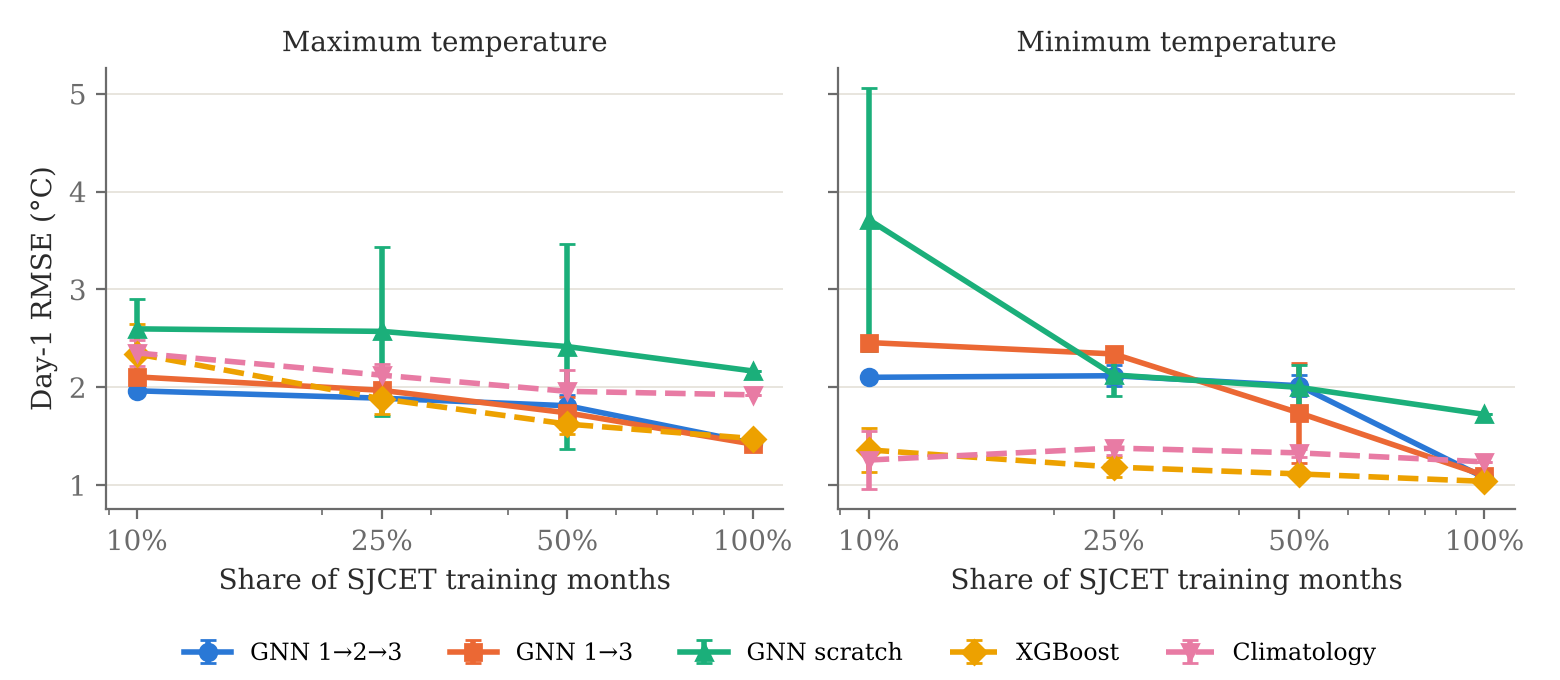
\includegraphics[width=0.98\textwidth]{data_efficiency.png}
    \caption{\capFigEfficiency}\label{fig:efficiency}
\end{figure}

\begin{table}[!htbp]
    \centering
    \caption{\capTabAblation}\label{tab:ablation}
    \footnotesize
    \begin{tabularx}{\textwidth}{|L{3.6cm}|C{1.35cm}|C{1.35cm}|C{1.35cm}|C{1.35cm}|Y|}
        \hline
        \textbf{Model} & \textbf{10\%} & \textbf{25\%} & \textbf{50\%} & \textbf{100\%} & \textbf{Variable} \\ \hline
        GNN 1$\to$\allowbreak{}2$\to$\allowbreak{}3 & \textbf{1.96} & 1.89 & 1.81 & 1.43 & \multirow{5}{*}{Tmax (\textdegree C)} \\ \cline{1-5}
        GNN 1$\to$\allowbreak{}3 & 2.11 & 1.97 & 1.74 & \textbf{1.42} & \\ \cline{1-5}
        GNN from scratch & 2.60 & 2.57 & 2.42 & 2.17 & \\ \cline{1-5}
        XGBoost & 2.34 & \textbf{1.88} & \textbf{1.62} & 1.48 & \\ \cline{1-5}
        Climatology & 2.35 & 2.12 & 1.96 & 1.92 & \\ \hline
        GNN 1$\to$\allowbreak{}2$\to$\allowbreak{}3 & 2.10 & 2.12 & 2.02 & 1.08 & \multirow{5}{*}{Tmin (\textdegree C)} \\ \cline{1-5}
        GNN 1$\to$\allowbreak{}3 & 2.46 & 2.34 & 1.74 & 1.10 & \\ \cline{1-5}
        GNN from scratch & 3.71 & 2.13 & 2.00 & 1.72 & \\ \cline{1-5}
        XGBoost & 1.36 & \textbf{1.18} & \textbf{1.11} & \textbf{1.04} & \\ \cline{1-5}
        Climatology & \textbf{1.26} & 1.38 & 1.33 & 1.24 & \\ \hline
    \end{tabularx}
\end{table}

\begin{itemize}
    \item \textbf{Four months of local data are enough for maximum temperature.} With 10\% of the months, the 1$\to$\allowbreak{}2$\to$\allowbreak{}3 model reaches 1.96\,\textdegree C, the best of all methods, against 2.60\,\textdegree C from scratch.
    \item \textbf{But not for minimum temperature.} With 10--50\% of the months, the pretrained GNNs are worse than climatology and XGBoost for Tmin (2.0--2.5 vs.\ 1.1--1.4\,\textdegree C), because SJCET's minimum varies very little and the network starts from a reanalysis minimum about 1.8\,\textdegree C too warm. This is the clearest negative result of the project.
    \item \textbf{The station stage helps only with little data} (1.96 vs.\ 2.11\,\textdegree C at 10\%); with six stations, none closer than about 50~km, its signal is weak.
\end{itemize}

\section{Live and Seasonal Performance}
\label{sec:res-livelike}

Because the register stops in 2016, a live forecast has no recent SJCET readings. Table~\ref{tab:livelike} scores the models with SJCET's own inputs hidden for the whole test period. The default model loses about 0.5\,\textdegree C on maximum temperature (1.43 to 1.98 at day 1) but hardly anything on minimum temperature (1.08 to 1.17), so the live forecast remains usable, and restoring SJCET's own inputs would recover most of the gap.

\begin{table}[!htbp]
    \centering
    \caption{\capTabLive}\label{tab:livelike}
    \footnotesize
    \begin{tabularx}{\textwidth}{|L{4.2cm}|C{1.7cm}|C{1.7cm}|C{1.7cm}|Y|}
        \hline
        \textbf{Model} & \textbf{Tmax d1} & \textbf{Tmax d6} & \textbf{Tmin d1} & \textbf{Tmin d6} \\ \hline
        GNN 1$\to$\allowbreak{}3 & \textbf{1.80} (1.42) & 1.90 (1.55) & \textbf{1.15} (1.10) & 1.21 (1.25) \\ \hline
        GNN 1$\to$\allowbreak{}2$\to$\allowbreak{}3 & 1.98 (1.43) & 2.05 (1.58) & 1.17 (1.08) & \textbf{1.20} (1.21) \\ \hline
        GNN from scratch & 2.21 (2.17) & \textbf{1.76} (1.85) & 1.63 (1.72) & 1.52 (1.43) \\ \hline
    \end{tabularx}
\end{table}

Table~\ref{tab:season} shows that temperature errors are smallest in the two monsoon seasons, when cloud cover keeps day-to-day changes small, and largest in winter and the pre-monsoon, which is also the season of isolated thunderstorms and the largest rain errors.

\begin{table}[!htbp]
    \centering
    \caption{\capTabSeason}\label{tab:season}
    \footnotesize
    \begin{tabularx}{\textwidth}{|L{4.4cm}|>{\centering\arraybackslash}X|>{\centering\arraybackslash}X|>{\centering\arraybackslash}X|>{\centering\arraybackslash}X|}
        \hline
        \textbf{Model / variable} & \textbf{Winter (Jan--Feb)} & \textbf{Pre-monsoon (Mar--May)} & \textbf{SW monsoon (Jun--Sep)} & \textbf{NE monsoon (Oct--Dec)} \\ \hline
        GNN 1$\to$\allowbreak{}2$\to$\allowbreak{}3, Tmax & 1.85 & 1.52 & 1.24 & 1.22 \\ \hline
        GNN 1$\to$\allowbreak{}2$\to$\allowbreak{}3, Tmin & 1.50 & 1.19 & 0.72 & 0.98 \\ \hline
        GNN 1$\to$\allowbreak{}2$\to$\allowbreak{}3, rain (mm) & 4.1 & 30.3 & 15.6 & 18.8 \\ \hline
        GNN scratch, Tmax & 2.34 & 2.89 & 1.67 & 1.57 \\ \hline
        GNN scratch, Tmin & 1.87 & 2.48 & 0.84 & 1.40 \\ \hline
    \end{tabularx}
\end{table}

\section{Application Interface}
\label{sec:res-app}

The forecasts, the digitized register and the model comparison are presented through a React web application backed by a FastAPI service. The \textbf{Forecast} page shows the live forecast for the coming days and lets a user replay any 2015--2016 date to compare the six-day forecast with what the register recorded, alongside the weather-network map (Figure~\ref{fig:app-forecast}). The \textbf{History} page shows the digitized register as a coverage heat-map, daily readings, and monthly and annual rainfall (Figure~\ref{fig:app-history}). The \textbf{Results} page presents the accuracy and error comparisons of this chapter interactively (Figure~\ref{fig:app-results}).

\begin{figure}[!htbp]
    \centering
    \IfFileExists{figures/app_forecast.png}{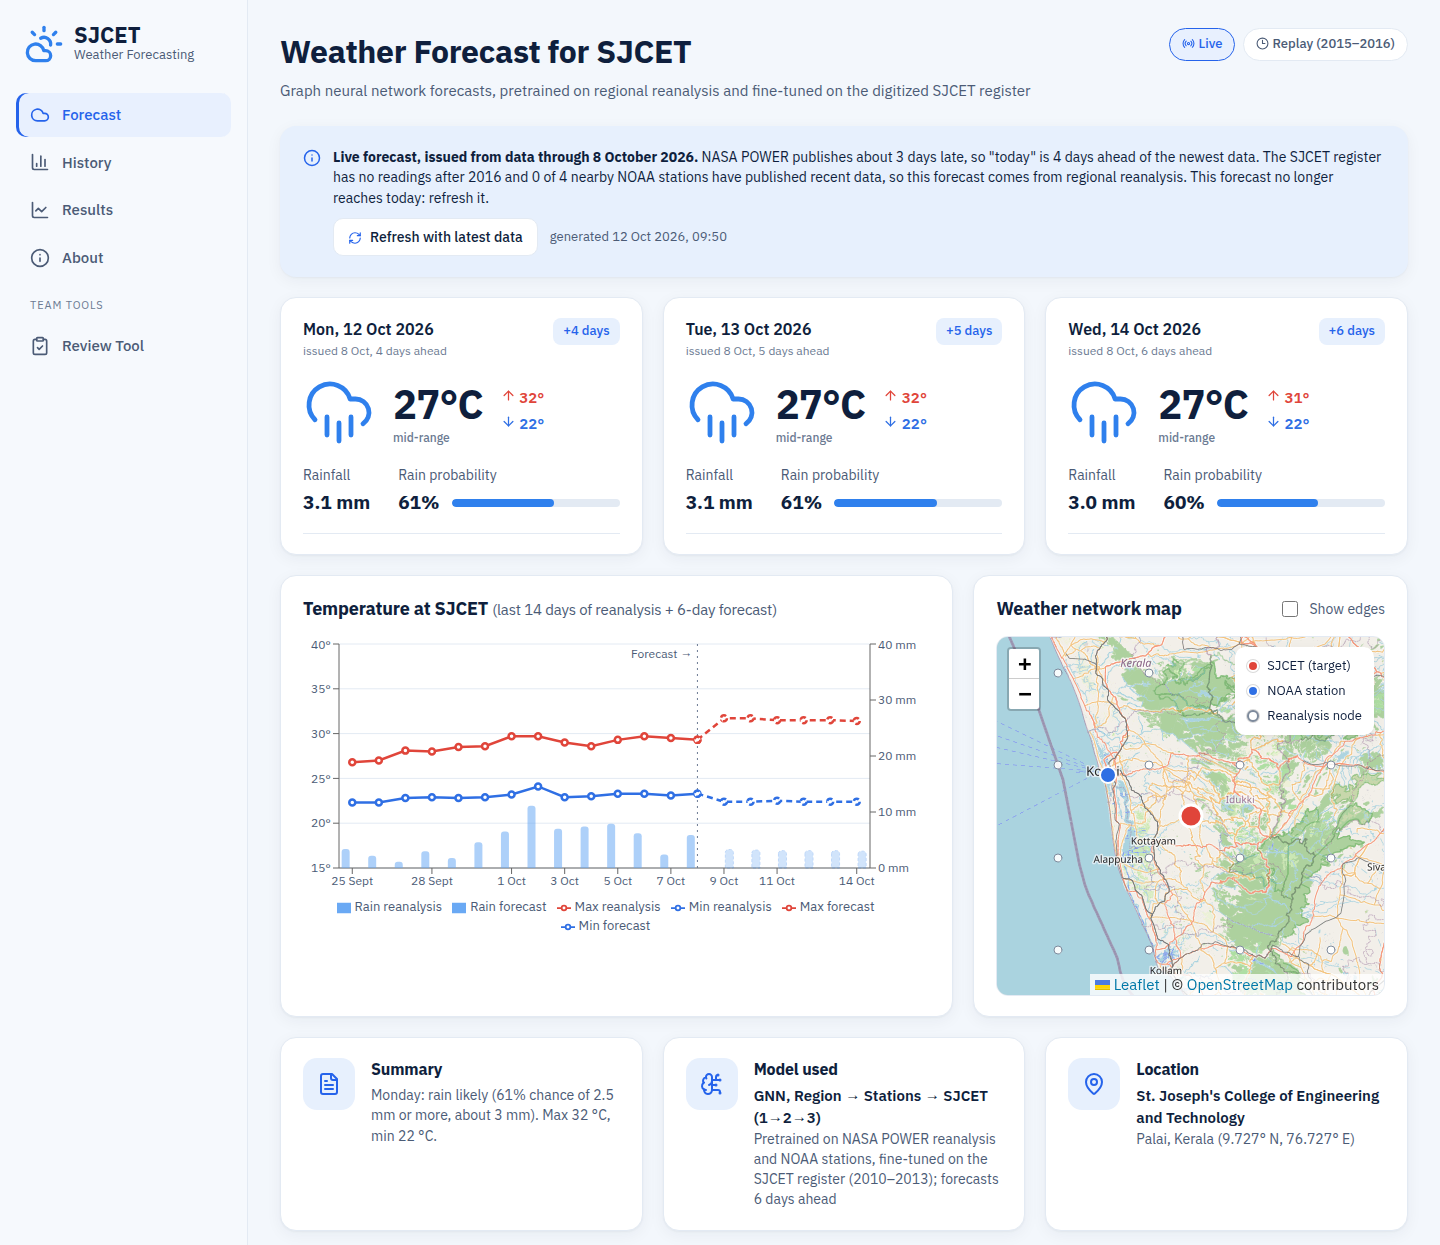
\includegraphics[width=0.9\textwidth]{app_forecast.png}}{\fbox{\parbox[c][5cm][c]{0.85\textwidth}{\centering Screenshot to be added: \textbf{figures/app\_forecast.png}}}}
    \caption{\capFigAppForecast}\label{fig:app-forecast}
\end{figure}

\begin{figure}[!htbp]
    \centering
    \IfFileExists{figures/app_history.png}{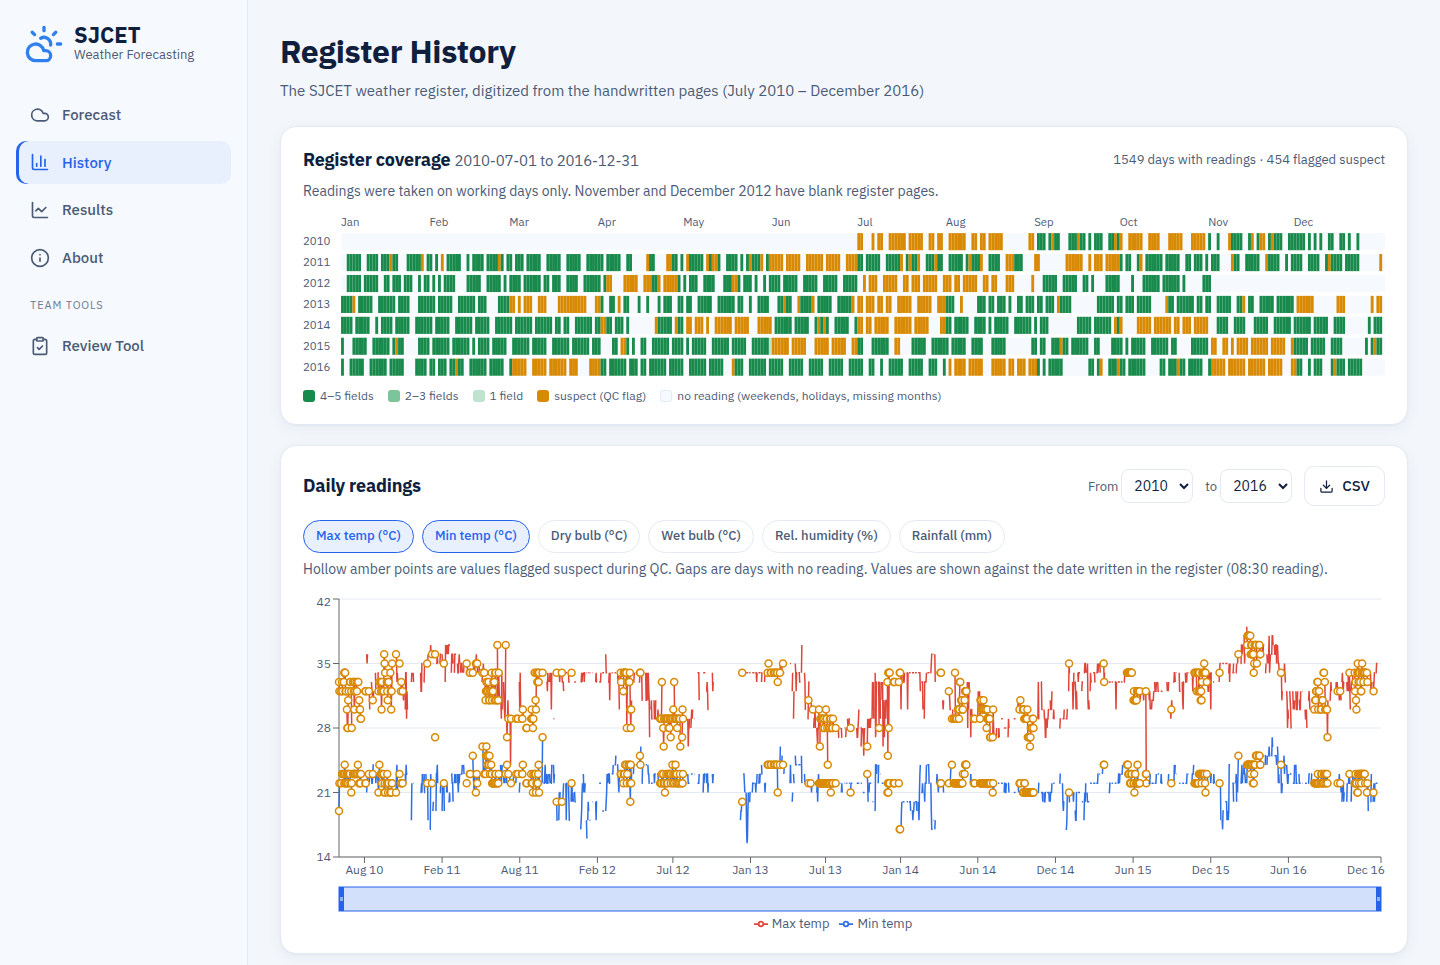
\includegraphics[width=0.9\textwidth]{app_history.png}}{\fbox{\parbox[c][5cm][c]{0.85\textwidth}{\centering Screenshot to be added: \textbf{figures/app\_history.png}}}}
    \caption{\capFigAppHistory}\label{fig:app-history}
\end{figure}

\begin{figure}[!htbp]
    \centering
    \IfFileExists{figures/app_results.png}{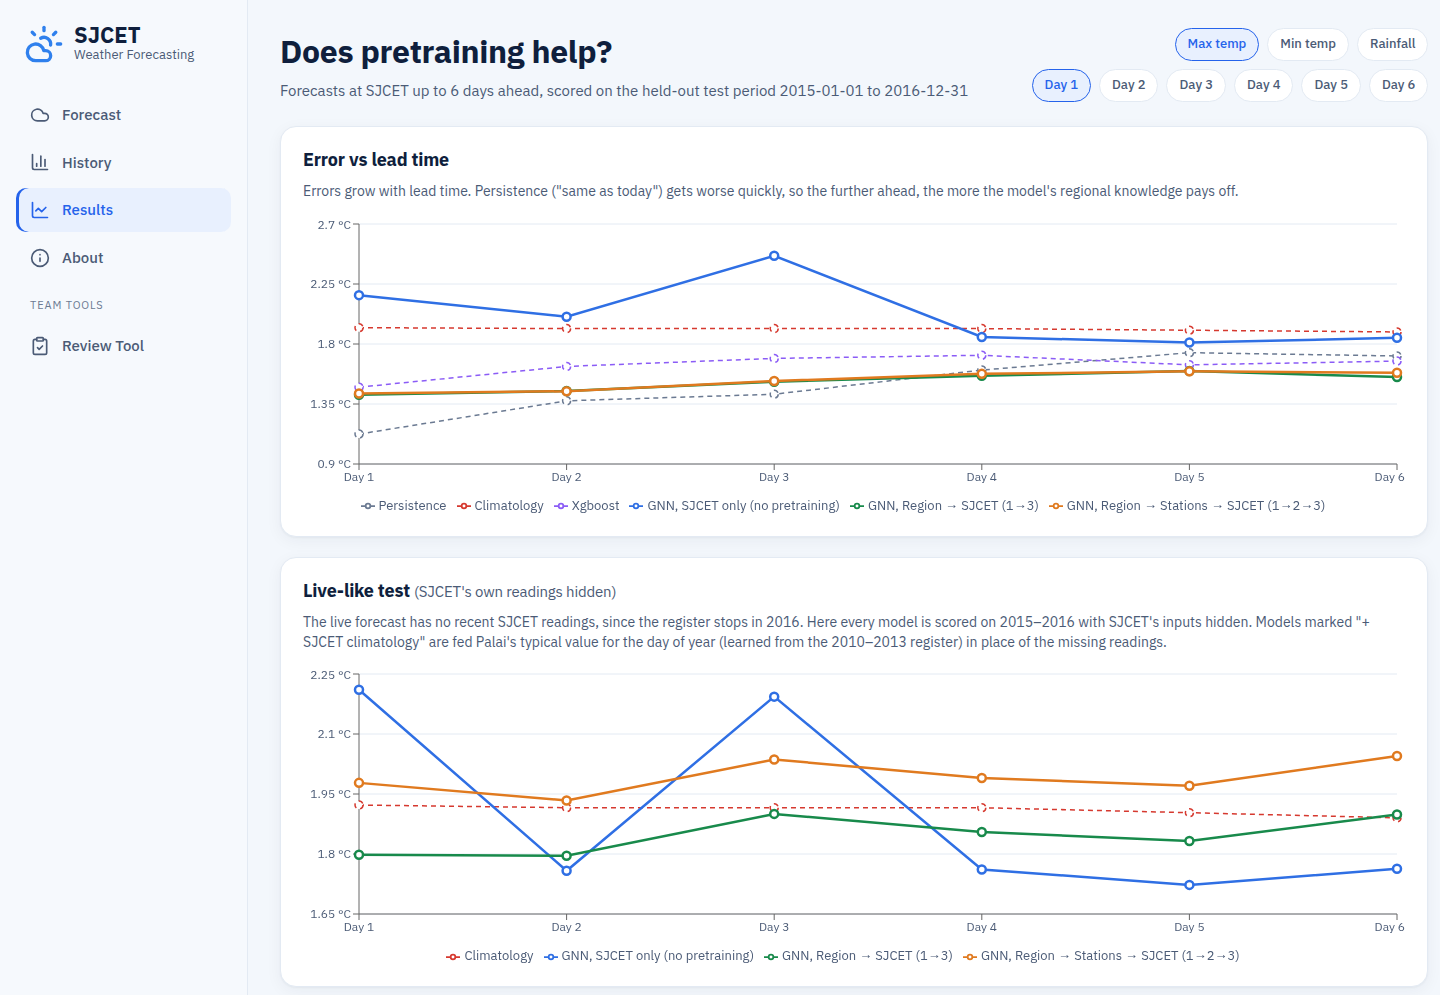
\includegraphics[width=0.9\textwidth]{app_results.png}}{\fbox{\parbox[c][5cm][c]{0.85\textwidth}{\centering Screenshot to be added: \textbf{figures/app\_results.png}}}}
    \caption{\capFigAppResults}\label{fig:app-results}
\end{figure}

\section{Summary of Observations}
\label{sec:res-summary}

\begin{itemize}
    \item The handwritten register was digitized into 1,549 traceable daily records, with 59 of 78 months confirmed against the observers' own totals.
    \item The final model forecasts next-day maximum and minimum temperature with 96.6\% and 96.2\% accuracy, with 86\% and 93\% of forecasts within $\pm$2\,\textdegree C.
    \item Pretraining on regional data lowers the temperature error by about a third and lets the model adapt to SJCET in only two epochs.
    \item With only four months of local data, the pretrained model is the best of all methods for maximum temperature, but worse than climatology for minimum temperature.
    \item The forecast remains usable without SJCET's own recent readings, losing about 0.5\,\textdegree C on maximum temperature.
    \item Rainfall at a single gauge remains the weakest part of the system.
\end{itemize}

\section{Discussion}
\label{sec:discussion}

The Phase 1 results show that staged transfer learning makes a modern forecasting model practical for a station with only a few years of handwritten data. Pretraining on regional reanalysis supplies the weather dynamics, and fine-tuning on the register supplies the local correction from the grid cell to the campus thermometer; together they produce temperature forecasts with about 96\% accuracy. The project's peculiarities shape these results in both directions: the register's whole-degree, often-repeated readings make persistence a hard baseline at one day, and the low variability of the minimum temperature makes climatology hard to beat when local data is scarce.

These conclusions rest on a small test set of a few hundred weekday readings, a reanalysis that carries its own biases, and a single station, so differences of a few hundredths of a degree should not be read as meaningful. In the next phase, the post-2016 photographs will be transcribed to lengthen the record and restore SJCET's inputs to the live forecast, the pretrained model will be combined with the station climatology for low-variance variables, and more and closer reference stations will be added to test the station stage properly.

\begin{thebibliography}{99}
\addcontentsline{toc}{chapter}{\numberline{}References}

\bibitem{ref1} E. Hawkins et al., ``Rescuing historical weather observations improves quantification of severe windstorm risks,'' \textit{Natural Hazards and Earth System Sciences}, vol. 23, pp. 1465--1482, 2023, doi: 10.5194/nhess-23-1465-2023.

\bibitem{ref2} L. G. Singh and S. E. Middleton, ``Data rescue of historical tables through semi-supervised table structure recognition,'' \textit{International Journal on Document Analysis and Recognition}, vol. 29, pp. 429--445, 2026, doi: 10.1007/s10032-025-00562-6.

\bibitem{ref3} L. G. Singh and S. E. Middleton, ``Tabular context-aware optical character recognition and tabular data reconstruction for historical records,'' \textit{International Journal on Document Analysis and Recognition}, vol. 28, pp. 357--376, 2025, doi: 10.1007/s10032-025-00543-9.

\bibitem{ref4} S. Raja, A. Mondal, and C. V. Jawahar, ``From pixels to tables: reconstructing complex tables from document images,'' \textit{International Journal on Document Analysis and Recognition}, 2025, doi: 10.1007/s10032-025-00553-7.

\bibitem{ref5} K. Bi, L. Xie, H. Zhang, X. Chen, X. Gu, and Q. Tian, ``Accurate medium-range global weather forecasting with 3D neural networks,'' \textit{Nature}, vol. 619, pp. 533--538, 2023, doi: 10.1038/s41586-023-06185-3.

\bibitem{ref6} L. Chen et al., ``FuXi: a cascade machine learning forecasting system for 15-day global weather forecast,'' \textit{npj Climate and Atmospheric Science}, vol. 6, Art. no. 190, 2023, doi: 10.1038/s41612-023-00512-1.

\bibitem{ref7} T. N. Nipen et al., ``Regional data-driven weather modeling with a global stretched grid,'' \textit{Artificial Intelligence for the Earth Systems}, vol. 5, no. 2, 2026, doi: 10.1175/AIES-D-25-0001.1.

\bibitem{ref8} S. K. Pal and D. Dutta, ``Transfer learning in weather prediction: Why, how, and what should,'' \textit{Journal of Computational and Cognitive Engineering}, vol. 3, no. 4, pp. 324--347, 2024, doi: 10.47852/bonviewJCCE42022817.

\bibitem{ref9} D. Prasad, A. Gadpal, K. Kapadni, M. Visave, and K. Sultanpure, ``CascadeTabNet: An approach for end to end table detection and structure recognition from image-based documents,'' in \textit{Proc. IEEE/CVF CVPR Workshops}, 2020, pp. 572--573.

\bibitem{ref10} B. Smock, R. Pesala, and R. Abraham, ``PubTables-1M: Towards comprehensive table extraction from unstructured documents,'' in \textit{Proc. IEEE/CVF CVPR}, 2022, pp. 4634--4642.

\bibitem{ref11} M. Li et al., ``TrOCR: Transformer-based optical character recognition with pre-trained models,'' in \textit{Proc. AAAI Conf. Artificial Intelligence}, vol. 37, no. 11, pp. 13094--13102, 2023.

\bibitem{ref12} A. Smith, N. Lott, and R. Vose, ``The Integrated Surface Database: Recent developments and partnerships,'' \textit{Bulletin of the American Meteorological Society}, vol. 92, no. 6, pp. 704--708, 2011, doi: 10.1175/2011BAMS3015.1.

\bibitem{ref13} S. Brody, U. Alon and E. Yahav, ``How attentive are graph attention networks?'' in \textit{Proc. International Conference on Learning Representations (ICLR)}, 2022.

\bibitem{ref14} T. Chen and C. Guestrin, ``XGBoost: a scalable tree boosting system,'' in \textit{Proc. 22nd ACM SIGKDD International Conference on Knowledge Discovery and Data Mining}, 2016, pp. 785--794, doi: 10.1145/2939672.2939785.

\bibitem{ref15} R. Gelaro et al., ``The Modern-Era Retrospective Analysis for Research and Applications, Version 2 (MERRA-2),'' \textit{Journal of Climate}, vol. 30, no. 14, pp. 5419--5454, 2017, doi: 10.1175/JCLI-D-16-0758.1.

\end{thebibliography}

%%%%%%%%%%%%%%%%%%%%%%%%%%%%%%%%%%%%%%%%%%%%%%%%%%%%%%%%%%%%%%%%%%%%%%%%%%%
%%%%%%%%%%%%%%%%%%           Appendices                   %%%%%%%%%%%%%%%%%
%%%%%%%%%%%%%%%%%%%%%%%%%%%%%%%%%%%%%%%%%%%%%%%%%%%%%%%%%%%%%%%%%%%%%%%%%%%%
\appendix
% list only the appendix titles in the contents
\addtocontents{toc}{\protect\setcounter{tocdepth}{0}}
\renewcommand{\thetable}{\thechapter.\arabic{table}}
\renewcommand{\chaptername}{Appendix}

\chapter{Sustainable Development Goal 13: Climate Action}
\label{app:sdg}

The project contributes to United Nations Sustainable Development Goal~13, \textbf{Climate Action: take urgent action to combat climate change and its impacts}. Climate change makes extreme weather more frequent and more severe, and adapting to it depends on knowing, at the local scale, how the weather has behaved in the past and how it is likely to behave in the coming days. Kerala, with two monsoons and sharp local differences across the Western Ghats, is a region where such local knowledge matters directly for agriculture, water supply and safety. The project contributes to SDG~13 in two ways: it \textbf{rescues a local climate record} that existed only on paper, and it \textbf{turns that record into a local forecast} using a method designed for places with little data.

\section{Contribution to the SDG 13 Targets}
\label{app:sdg-targets}

Table~\ref{tab:sdg} lists the SDG~13 targets that the work of Phase~1 supports, with the part of this report where the evidence is given.

\begin{table}[!htbp]
    \centering
    \caption{Contribution of the project to the targets of SDG~13.}\label{tab:sdg}
    \footnotesize
    \begin{tabularx}{\textwidth}{|L{3.6cm}|Y|L{2.6cm}|}
        \hline
        \textbf{SDG 13 target} & \textbf{Contribution of this project} & \textbf{Evidence} \\ \hline
        \textbf{13.1} Strengthen resilience and adaptive capacity to climate-related hazards and natural disasters &
        Six-day forecasts of maximum and minimum temperature and rainfall for the campus, made from the newest available data, so that heat and heavy rain can be anticipated locally. Next-day temperature accuracy is 96.6\% (maximum) and 96.2\% (minimum). &
        Sections~\ref{sec:res-accuracy} and~\ref{sec:res-livelike} \\ \hline
        \textbf{13.1} (continued) &
        A data-efficient method: staged transfer learning lets a station with only a few years of readings obtain a usable forecast, so the approach can be reused by schools, farms and small stations that have little local data. &
        Sections~\ref{sec:stages} and~\ref{sec:res-efficiency} \\ \hline
        \textbf{13.3} Improve education, awareness-raising and human and institutional capacity on climate change mitigation, adaptation, impact reduction and early warning &
        Rescue of close to twenty years of the college's handwritten weather register: 1,549 observed days from 2010--2016 digitized, validated against the observers' own monthly totals and preserved as a traceable dataset for studying the local climate. &
        Section~\ref{sec:digitization} \\ \hline
        \textbf{13.3} (continued) &
        A web application that presents the digitized history, the live forecast and the model comparison to students and staff, building awareness of the local climate and institutional capacity for early warning. &
        Section~\ref{sec:res-app} \\ \hline
    \end{tabularx}
\end{table}

\section{Planned Impact in Phase 2}
\label{app:sdg-phase2}

\begin{itemize}
    \item \textbf{Long-term local climate trends:} transcribing the register from 2017 onwards will extend the record towards twenty years and allow a study of how temperature and rainfall at the campus have changed.
    \item \textbf{Automatic weather station:} live readings from the campus will restore SJCET's own inputs to the forecast and support early warnings of heavy rain or extreme heat.
    \item \textbf{A reusable method:} the digitization and transfer-learning pipeline can be applied to other institutions in Kerala that hold paper weather records.
\end{itemize}

\chapter{Project Cost Estimation}
\label{app:cost}

This appendix estimates the cost of Phase~1 of the project as a professional software project, using the standard estimation equation
\[
\text{Total project cost}=(\text{Total effort in hours}\times\text{Hourly rate})+\text{Fixed overhead costs}+\text{Contingency}.
\]
The effort is divided into roles with separate hourly rates. The estimate represents the market value of the work; the actual expenditure in Phase~1 was small, because all data sources and software are free and the work was done on the team's own laptops.

\section{Work Breakdown and PERT Estimation}
\label{app:cost-wbs}

The work of Phase~1 is broken into twelve tasks (Table~\ref{tab:wbs}). For each task, an optimistic ($O$), most likely ($M$) and pessimistic ($P$) effort in hours is estimated, and the expected effort is computed with the three-point (PERT) formula
\[
\text{Estimated hours}=\frac{O+4M+P}{6}.
\]

\begin{table}[!htbp]
    \centering
    \caption{Work breakdown structure with three-point (PERT) effort estimates, in hours.}\label{tab:wbs}
    \footnotesize
    \begin{tabularx}{\textwidth}{|C{0.6cm}|Y|L{2.7cm}|C{0.8cm}|C{0.8cm}|C{0.8cm}|C{1.3cm}|}
        \hline
        \textbf{No.} & \textbf{Task} & \textbf{Role} & \textbf{O} & \textbf{M} & \textbf{P} & \textbf{PERT} \\ \hline
        1 & Literature survey and requirement analysis & ML/Data Engineer & 20 & 30 & 45 & 30.8 \\ \hline
        2 & Transcription of the register (78 months) & Data Annotator & 40 & 60 & 90 & 61.7 \\ \hline
        3 & Validation, rainfall checksums and dataset assembly & ML/Data Engineer & 6 & 10 & 16 & 10.3 \\ \hline
        4 & OCR prototyping and evaluation (TrOCR, GloSAT) & ML/Data Engineer & 8 & 12 & 20 & 12.7 \\ \hline
        5 & Regional data acquisition and weather-graph construction & ML/Data Engineer & 8 & 12 & 20 & 12.7 \\ \hline
        6 & GNN model, staged training, ablation and baselines & ML/Data Engineer & 20 & 30 & 50 & 31.7 \\ \hline
        7 & Evaluation and live forecasting & ML/Data Engineer & 6 & 10 & 16 & 10.3 \\ \hline
        8 & UI/UX design of the web application & UI/UX Designer & 6 & 10 & 16 & 10.3 \\ \hline
        9 & Backend API and frontend development & Software Engineer & 12 & 20 & 32 & 20.7 \\ \hline
        10 & Testing, verification and reproduction of results & QA / Tester & 8 & 12 & 20 & 12.7 \\ \hline
        11 & Project management, reviews and coordination & Project Manager & 15 & 20 & 30 & 20.8 \\ \hline
        12 & Documentation and report preparation & Technical Writer & 25 & 35 & 50 & 35.8 \\ \hline
        \multicolumn{6}{|r|}{\textbf{Total estimated effort}} & \textbf{270.5} \\ \hline
    \end{tabularx}
\end{table}

The software development effort is modest because the code was written with modern AI-assisted development tools and builds on open-source libraries (PyTorch Geometric, FastAPI, React), and because model training runs unattended on a CPU, so machine time is not counted as working hours. The largest manual tasks are transcribing the paper register and preparing the documentation.

\section{Team Composition and Labour Cost}
\label{app:cost-labour}

Table~\ref{tab:roles} groups the effort by role and applies an hourly rate to each role. The rates are entry-level rates for each role.

\begin{table}[!htbp]
    \centering
    \caption{Effort and labour cost by role.}\label{tab:roles}
    \footnotesize
    \begin{tabularx}{\textwidth}{|Y|C{1.8cm}|C{1.9cm}|C{2.3cm}|C{2.4cm}|}
        \hline
        \textbf{Role} & \textbf{Hours} & \textbf{Share of effort} & \textbf{Rate (\rupee/hour)} & \textbf{Cost (\rupee)} \\ \hline
        ML/Data Engineer & 108.5 & 40.1\% & 550 & 59,675 \\ \hline
        Software Engineer & 20.7 & 7.7\% & 450 & 9,315 \\ \hline
        UI/UX Designer & 10.3 & 3.8\% & 400 & 4,120 \\ \hline
        QA / Tester & 12.7 & 4.7\% & 350 & 4,445 \\ \hline
        Project Manager & 20.8 & 7.7\% & 500 & 10,400 \\ \hline
        Data Annotator & 61.7 & 22.8\% & 200 & 12,340 \\ \hline
        Technical Writer & 35.8 & 13.2\% & 350 & 12,530 \\ \hline
        \textbf{Total} & \textbf{270.5} & \textbf{100\%} & & \textbf{1,12,825} \\ \hline
    \end{tabularx}
\end{table}

Engineering work (ML/data and software) accounts for 47.8\% of the effort, slightly below the usual 50--60\% for software projects, and UI/UX design, testing and project management take smaller shares than in a typical application project. This reflects the nature of the project: it is research-oriented, the development work was accelerated by AI-assisted tools, and a large part of the effort goes to data, with the hand transcription of the paper register alone accounting for 22.8\% of the hours.

\section{Overheads, Contingency and Total Cost}
\label{app:cost-total}

Infrastructure and third-party costs are low because every data source and tool used in Phase~1 is free: NASA POWER and NOAA GSOD data, OpenStreetMap tiles, and open-source software (Python, PyTorch, FastAPI, React, \LaTeX). Training runs on a CPU, so no GPU or cloud training is needed. The remaining overheads, the contingency buffer of 15\% and the total are given in Table~\ref{tab:cost}.

\begin{table}[H]
    \centering
    \caption{Total estimated cost of Phase~1.}\label{tab:cost}
    \footnotesize
    \begin{tabularx}{\textwidth}{|Y|C{3.0cm}|}
        \hline
        \textbf{Item} & \textbf{Cost (\rupee)} \\ \hline
        Labour (Table~\ref{tab:roles}) & 1,12,825 \\ \hline
        Cloud hosting for the web application (small virtual machine, 4 months $\times$ \rupee1,500) & 6,000 \\ \hline
        Domain name (one year) & 1,000 \\ \hline
        Internet and electricity (share for the project) & 4,000 \\ \hline
        Printing and binding of reports & 2,000 \\ \hline
        Third-party data and APIs (NASA POWER, NOAA GSOD, OpenStreetMap) & 0 \\ \hline
        \textbf{Subtotal} & \textbf{1,25,825} \\ \hline
        Contingency (15\% of subtotal) & 18,874 \\ \hline
        \textbf{Total estimated cost} & \textbf{1,44,699} \\ \hline
    \end{tabularx}
\end{table}

The estimated cost of Phase~1 is therefore about \textbf{\rupee1.45 lakh} for about 270 hours of effort. This is below the minimum-viable-product band of industry benchmarks (400--700 hours, \rupee2,00,000--\rupee3,50,000), because the free open-data stack removes almost all infrastructure cost and AI-assisted development shortens the coding effort. Phase~2 will add the cost of the automatic weather station and of transcribing the remaining records.

% \newpage
\markboth{References}{}
\fancyhead{}
\fancyfoot{}


\renewcommand{\footrulewidth}{0pt}
\renewcommand{\headrulewidth}{0pt}
\newcommand{\wideunderline}[2][2em]{%
  \underline{\makebox[\ifdim\width>#1\width\else#1\fi]{#2}}%
}
\begin{center}
% \pagestyle{none}
 \vspace*{1cm}
    \Large \textbf{ VISION \& MISSION OF THE DEPARTMENT}
     \vspace*{2.0cm}
\\ {\Large \bf \wideunderline[12em]{Vision}}
 \\ \vspace{1.0cm}
 {\normalsize To achieve excellence in Artificial Intelligence and Data Science to cater 
 to the ever-changing industrial and socio-economic needs.} 

 \vspace*{2.0cm}

 % Mission Section
 {\Large \bf \wideunderline[12em]{Mission}}
 \\ \vspace{1.0cm}
 \begin{itemize}
   \item \normalsize To provide high-quality and value-based technical education in the Artificial Intelligence and Data Science program.
   \item \normalsize To establish an infrastructure fostering industry-institute interaction in order to meet global expectations and requirements.
   \item \normalsize To empower students to become globally competent and effective problem-solvers to develop entrepreneurial skills and pursue higher studies.
 \end{itemize}

\end{center}

\end{document}
